% Chapter 4

\chapter{Validation Expérimentale } % Main chapter title

\label{Chapter4} % For referencing the chapter elsewhere, use \ref{Chapter1} 

%----------------------------------------------------------------------------------------

\section{Introduction}
Les expérimentations sont essentielles pour la validation de nos algorithmes et approches, cette étape nécessite de déterminer les caractéristiques des machines utilisées ainsi que la description de la partie logiciel dont nous avons eu besoin, mais surtout une bonne organisation des expérimentations. C'est justement l'objet de ce chapitre, qui est structuré comme suit:\\
 $-$ Description de l'environnement de développement.\\
 $-$ Expérimentations, dont l'organisation détaillée suivie des résultats obtenus regroupé par types d'environnements et par types d'expérimentations.\\
 $-$ Présentation du simulateur accompagné de son manuel d'utilisation.


\section{Environnement de développement}
Comme pour toute expérimentation l'environnement de test est un élément clé pour la bonne interprétation des résultats obtenus.

\subsection{Matériel}
Nous avons utilisé deux machines (Laptop) possédant les caractéristiques et capacités suivantes:

 
\noindent
\fbox{\parbox{\textwidth}{
		
\begin{multicols}{2}
\begin{minipage}[t]{0.45\textwidth}
	\underline{\textbf{Machine 1 :}}
	\vspace{0.2cm}
	\begin{description}
		\item[Mémoire RAM:] 8 Go
		\item[Processeur:] Intel® Core™ i5-6200U CPU  2.30GHz x 4 
		\item[Carte graphique:] Intel® HD Graphics 520 (Skylake GT2) x86/MMX/SSE2
		\item[Type de l'OS:] UBUNTU 14.04 LTS  32-bit
	\end{description}
\end{minipage}\hfill

	\columnbreak
\begin{minipage}[t]{0.45\textwidth}
	\underline{\textbf{Machine 2 : }}
	\begin{center}
		\begin{description}
			\item[Mémoire RAM:] 8 Go
			\item[Processeur:] Intel® Core™ i5-3317U  @ 1.70Hz  1.70GHz
			\item[Carte graphique:] Intel® HD Graphics 520 \hspace{5.5cm}  \textbf{        .}
			\item[Type de l'OS:] UBUNTU 18.04 LTS  64-bit
		\end{description}
		
	\end{center}
\end{minipage}\hfill

\end{multicols}
}}

\subsection{Logiciels}
Le développement de nos algorithmes a été exclusivement fait sous système d'exploitation \textbf{Linux} (\textit{Ubuntu}), celui-ci muni des logiciels suivants:
\paragraph{Intellij IDEA}
 est un environnement de développement de logiciel informatique orienté \textbf{Java}, supportant une large palette de plugins. C'est un des nombreux produits développés par la compagnie \textit{JetBrains}. celle-ci nous a été mise à disposition via une licence étudiant.
 
 Nous l'avons utilisé pour le développement de notre solution de recherche de cible.

\paragraph{- Java}  est un langage orienté objet académique qui a fait ses preuves, très largement utilisé pour ses nombreux avantages dont on cite: la portabilité,
large diversité des librairies, conséquente documentation, ...etc

Nous avons eu recours à une bibliothèque seulement, cela pour l'interface graphique en (\textbf{javaFx}) de notre simulateur en Java 
\paragraph{jfoenix-8.0.8.jar} JFoenix\footnote{Lien : https://github.com/jfoenixadmin/JFoenix} est une librairie mettant à disposition des composantes java qui implémentent Google Material Design, elle est open source, et dédiée aux applications java, spécialement les interfaces \textit{javaFx}. 


\paragraph{PyCharm}
est un environnement de développement de logiciel informatique sous langage \textbf{Python}, aussi fournis par la compagnie \textit{JetBrain} que nous avons obtenu sous licence étudiant.
Nous l'avons principalement utilisé pour exploiter les résultats des expérimentations pour les traiter et traduire en graphe plus significatifs.

\paragraph{Python} est un langage de programmation interprété qui a plus ou moins récemment fait surface et qui est de plus en plus utilisé depuis surtout en vu de sa simplicité et polyvalence.










%\newpage

\section{Expérimentations}
L'organisation des expérimentations étant très importante pour la comparaison des résultats de manière effective, nous les avons établis selon les étapes suivantes:

\begin{enumerate}
	\item Paramétrer notre mini algorithme génétique (GA) : à travers cette étape nous avons obtenu les paramètres suivants:
		\subitem $\bullet$ Taille de la population : 20
		\subitem $\bullet$ Nombre d'itération : 30
		\subitem $\bullet$ Nombre de mutation : 2
		\subitem $\bullet$ Point de croisement : aléatoire
	
	\item Pour chaque taille d'environnement / portée des cibles / nombre de cibles nous avons paramétré nos Algorithmes de recherche (BSO, MBSO, ESWSA, EHO) à l'aide de l'algorithme génétique (GA), la moyenne des 5 meilleurs paramètres obtenus sera sélectionné comme meilleur paramètre de la méthode, nous présentant ces paramètres en détails dans l'annexe \ref{AppendixB}.
	
	\item Puis pour chaque type\footnote{type : environnement avec une taille, une portée et un nombre de cible données.} d'environnement nous avons effectué la recherche de cible avec nos algorithmes (BSO, MBSO, EHO, ESWSA) sur quatre (4) différents environnements, en exécutant 10 fois chacun.\\
	Ce qui revient à 40 exécution par type  d'environnement dont nous ferons la moyenne.
	
	\item Tous les résultats obtenus ont été enregistrés: Nombre d'itération, temps d'exécution, taux de succès %\footnote{complexité : nombre d'itération $\times$ nombre de robot utilisé}
	 ainsi que paramètres utilisés pour chaque méthode.
\end{enumerate}

Les résultats de nos expérimentations sont classés par rapport à la densité des obstacles dans l'environnement (Sans obstacle, avec obstacle et complexe), tels que chacun est composé de 3 parties selon le type d'expérimentation (taille d'environnement , portée des cibles et nombre de cibles), sachant que les deux premiers comporte 2 variantes le mono-cible (1 cible) ainsi que la multi-cible (5 cibles).

\subsection{Organisation des types d'expérimentations}
Pour une question de clarté, nous avons jugé nécessaire de décrire comment est organisé chaque type d'expérimentation avons de passer aux résultats obtenus.

\subsubsection{Expérimentation par rapport à la portée des cibles}
Pour les expérimentations par rapport à l'influence de la portée des cibles sur le comportement de nos algorithmes de recherche, nous avons fixé la taille de l'environnement à 500 $\times$ 500 positions et fait varier la portée d'un rayon de 10 positions à 100 positions avec un pas de 10.

Ainsi comme le montre la figure \ref{orgPortee}, les tests de ce type proviennent des exécutions sur 40 environnements (4 par portée), soit 400 exécutions pour le mono-cible et 400 autres pour le multi-cible, pour chaque méta-heuristique (après paramétrage).

\begin{center}	 
	\captionsetup{width=1\linewidth} 
	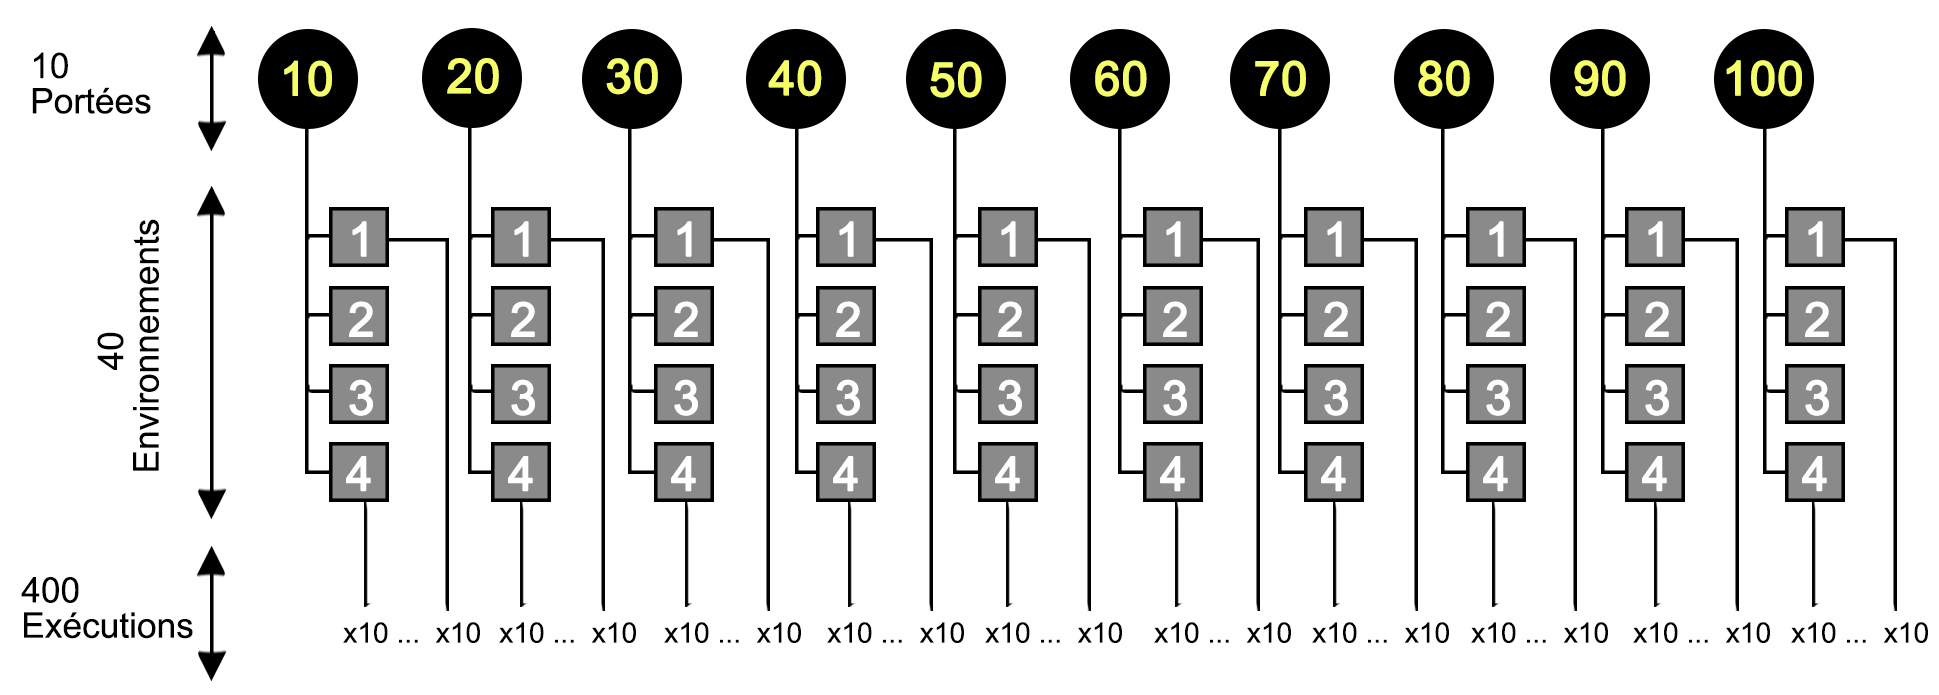
\includegraphics[width=0.7\textwidth]{org-portee.jpg}%
	\vspace{-0.1 cm}
	\captionof{figure}{Représentation de l'organisation des expérimentations sur la portée des cibles.}\label{orgPortee}%
\end{center}

\subsubsection{Expérimentation par rapport à la taille de l'environnement}
Pour les expérimentations sur l'influence de la taille de l'environnement sur le comportement de nos méta-heuristiques pour la recherche de cibles, nous avons adapté la portée des cibles à chaque taille d'environnement conformément à l'équation suivante:
\begin{equation}
portee = \frac{taille_{Cot\acute{e}} \times 10}{100} = \frac{taille_{Cot\acute{e}}}{10}
\label{porteeEnv}
\end{equation}	
Ce qui revient à :
\begin{equation}	
S_{cible} = \frac{\sqrt{S_{env}}}{5} \times \pi
\end{equation}

Avec :
\begin{itemize}
	\item[$-$] $taille_{Cot\acute{e}}$ : taille du coté de l'environnement carré.
	\item[$-$] $S_{cible}$ : surface d'émission de la cible (rayon = portée).
	\item[$-$] $S_{env}$ : surface de l'environnement de recherche ($S_{env}$ = $taille_{Cot\acute{e}}$).\\
\end{itemize}

Pour cela nous avons sélectionné dix différentes tailles d'environnement, les tailles du coté de ces environnements sont comme suit : 50, 100, 200, 400, 600, 800, 1000, 1500, 3000, 5000.

les surfaces respectives sont les suivantes: 2500, 10000, 40000, 160000, 360000, 640000, 1000000, 2250000, 9000000, 25000000.

Ainsi les portées correspondantes sont: 5, 10, 20, 40, 60, 80, 100, 150, 300, 500.


\textbf{ }\\
Les résultats des testes liés à ce type sont le résultat de 40 exécutions par taille d'environnement (4 configurations pour chaque taille), ce qui revient à un total de 400 exécutions pour le mono-cible et 400 autres pour le multi-cible, et ce pour chaque approche (après paramétrage). Le schéma \ref{orgSize} ci-dessous illustre cette organisation.

\begin{center}	  
	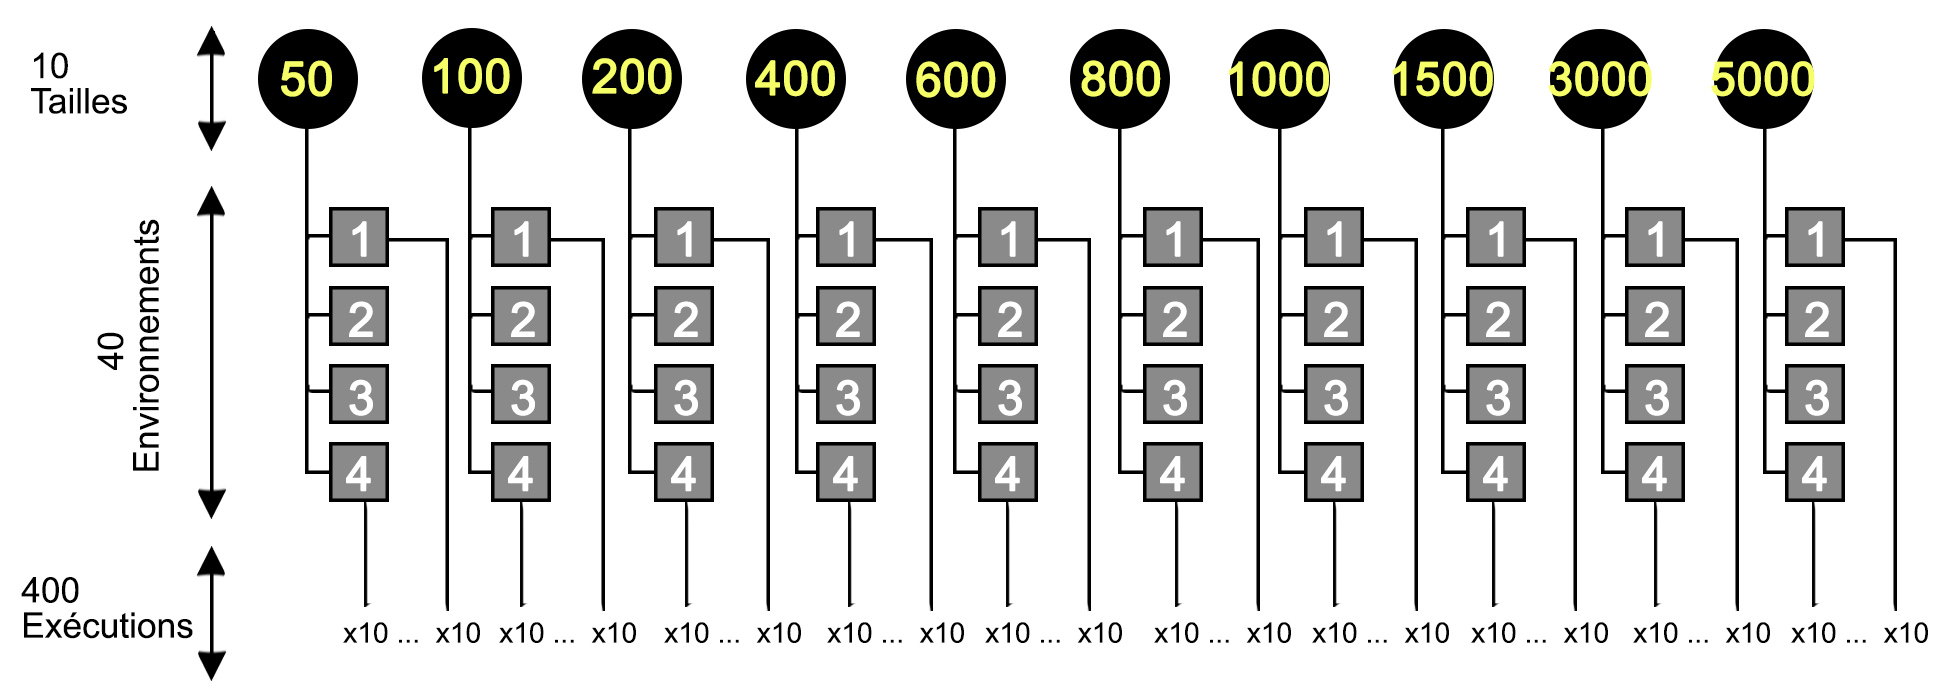
\includegraphics[width=0.75\textwidth]{org-size.jpg}%
	\vspace{-0.1 cm}
	\captionof{figure}{Représentation de l'organisation des expérimentations sur la taille des environnements.}\label{orgSize}%
\end{center}

\subsubsection{Expérimentation par rapport au nombre de cible}
Ces expérimentations permettent d'étudier l'influence du nombre de cibles présentes dans nos environnements sur le comportement de nos métaheuristiques (BSO, EHO, ESWSA et MBSO).
Pour cela nous avons fixé la taille des environnements à 500 $\times$ 500 positions ainsi qu'une portée de cible égale à 50 (conformément à l'équation \ref{porteeEnv}).\\

Nous avons pris le nombre de variable compris entre 1 et 15 (bornes incluent) avec un pas de 2, ce qui nous donne les 8 nombres de cibles suivants : 1, 3, 5, 7, 9, 11, 13, 15.\\

De ce fait, les résultats des tests sont le fruit d'exécution sur 32 environnements (4 par nombre de cible) , ce qui correspond à 320 exécutions pour chacune des approches développées (après paramétrage).\\
La figure \ref{orgNbrT} ci-dessous schématise cette organisation:

\begin{center}	  
	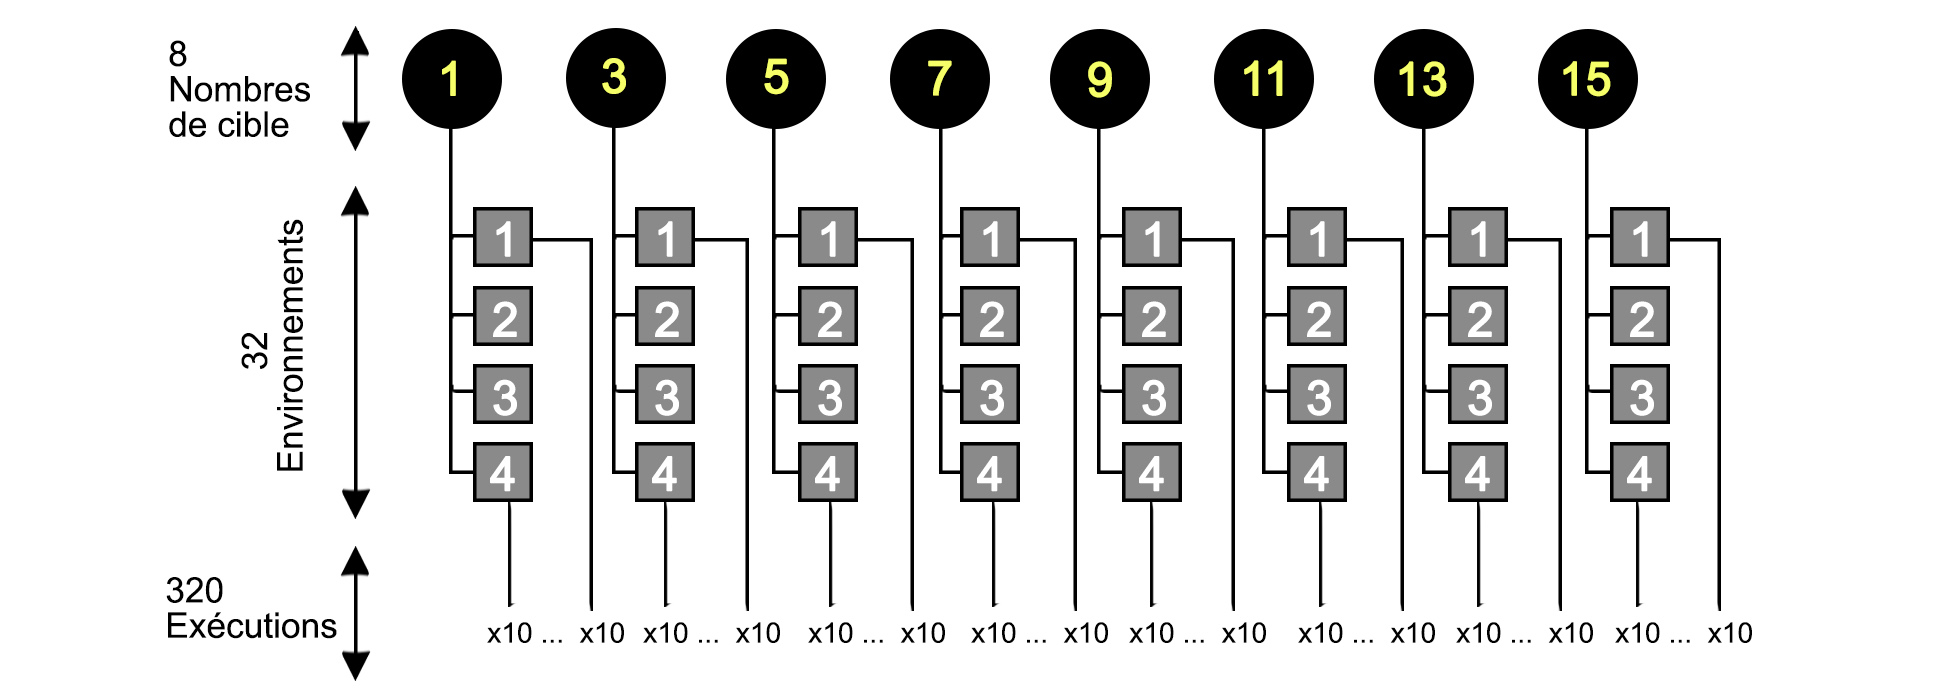
\includegraphics[width=0.8\textwidth]{org-nbrT.jpg}%
	\vspace{-0.1 cm}
	\captionof{figure}{Représentation de l'organisation des expérimentations sur le nombre de cible.}\label{orgNbrT}%
\end{center}



% \newpage
 
 %%%%%%%%%%%%%%%%%%%%%%%%%%%%%%%%%%%%%%%%%%%%%%%%%%%%
 
\subsection{Environnement sans obstacles}
\subsubsection{Expérimentation par rapport à la portée des cibles}

\paragraph{- Mono-cible}
\textbf{ }\\
Les expérimentations qui suivent, portent sur le nombre moyen d'itérations par exécution, le temps moyen ainsi que le taux moyen de succès à trouver la cible selon sa portée.

%\newpage 

%\paragraph{ }
%\begin{table}[h]
%	\begin{tabular}{p{1.5cm}*{80}{@{\hskip1.5mm}c@{\hskip1.5mm}}}
%		\toprule
%		\textbf{P} &   &
%		\multicolumn{3}{l}{\textbf{EHO}} &  &
%		\multicolumn{3}{l}{\textbf{ESWSA}} &  &
%		\multicolumn{3}{l}{\textbf{BSO}} &  &
%		\multicolumn{3}{l}{\textbf{MBSO}}\\
%		\cline{3-5}\cline{7-9}\cline{11-13}\cline{15-17}	& & 
%		
%		Itér & Tps & \%R &  &
%		Itér & Tps & \%R &  &
%		Itér & Tps & \%R &  &
%		Itér & Tps & \%R \\ 
%		\hline
%		10 & & 12.03 & 0.04 & 100 & & 13.38 & 0.02 & 100 & & 32.98 & 0.02 & 100 & & 16.30 & 0.01 & 100 \\ 20 & & 7.83 & 0.02 & 100 & & 9.00 & 0.02 & 100 & & 21.78 & 0.01 & 100 & & 7.18 & 0.00 & 100 \\ 30 & & 3.93 & 0.01 & 100 & & 3.90 & 0.01 & 100 & & 19.33 & 0.01 & 100 & & 8.13 & 0.01 & 100 \\ 40 & & 4.48 & 0.02 & 100 & & 7.40 & 0.02 & 100 & & 18.95 & 0.01 & 100 & & 6.93 & 0.01 & 100 \\ 50 & & 3.78 & 0.02 & 100 & & 2.53 & 0.02 & 100 & & 11.70 & 0.01 & 100 & & 6.55 & 0.01 & 100 \\ 60 & & 4.20 & 0.02 & 100 & & 2.33 & 0.02 & 100 & & 11.80 & 0.01 & 100 & & 5.93 & 0.01 & 100 \\ 70 & & 1.70 & 0.02 & 100 & & 2.10 & 0.03 & 100 & & 8.20 & 0.01 & 100 & & 3.80 & 0.01 & 100 \\ 80 & & 2.30 & 0.03 & 100 & & 2.20 & 0.05 & 100 & & 8.20 & 0.01 & 100 & & 3.75 & 0.01 & 100 \\ 90 & & 2.35 & 0.03 & 100 & & 2.63 & 0.06 & 100 & & 8.60 & 0.01 & 100 & & 3.73 & 0.01 & 100 \\ 100 & & 1.35 & 0.05 & 100 & & 2.20 & 0.08 & 100 & & 4.98 & 0.02 & 100 & & 3.45 & 0.02 & 100 \\ 
%		\bottomrule
%	\end{tabular}
%	\captionsetup{width=1\linewidth}
%	\caption{Nombre d'itération moyen, temps d'exécution moyen et taux de succès dans un environnement sans obstacle avec différentes portées de la cible.}
%	\label{tabPortee1}
%\end{table}





%minipage text + graphe

\hspace{-0.5cm}
\begin{minipage}[t]{0.5\textwidth}
	\subparagraph{Taux de réussite}
	\textbf{  }\\
	
	La figure \ref{TP1} est un \textit{BarChart} représentant l'évolution du taux de réussite de chacune de nos métaheuristiques par rapport aux différentes portées de la cible dans un environnement sans obstacle.\\
	 
	Nous observons que n'importe la portée de notre cible allant de 10 à 100, nos quatre algorithmes obtiennent 100\% de réussite, c'est à dire arrivent toujours à trouver cette unique cible 
	dans la limite du nombre d'itérations maximal (1000).
	
\end{minipage}\hfill
\begin{minipage}[t]{0.55\textwidth}
	\captionsetup{width=0.8\linewidth}
	\centering\raisebox{\dimexpr \topskip-\height}{%
		\includegraphics[width=\textwidth]{SansObs/BarChart/TauxPortee1.pdf}}
	\vspace{-0.3cm}
	\captionof{figure}{Comparaison de la variation du taux de réussite des algorithmes selon la portée de la cible (sans obstacle).}
	\label{TP1}
\end{minipage}\hfill

\textbf{ }\\

\noindent
\paragraph{Variation du nombre d'itérations et temps d'exécution}
\textbf{ }\\

Les figures \ref{IP1} et \ref{tP1} sont des \textit{LineCharts}, représentant respectivement la variation du nombre d'itération et temps d'exécution de chacune de nos approches confrontées aux différentes portées de la cible dans un environnement sans obstacle.\\

Nous remarquons que toutes les méthodes voient leurs nombre d'itérations décroître avec l'augmentation de la portée de la cible. Pour les trois méthodes MBSO, EHO et ESWSA le nombre d'itération est estimé entre 12 et 16 pour une portée égale à 10 et décroît progressivement jusqu'à atteindre environ 2 ou 3 itérations pour la portée maximale, par contre BSO débute avec un peu plus d'itération (moyenne de 33), avant de diminuer pour rejoindre les autres méthodes lorsque la portée est de 100 positions.\\

Pour ce qui est des temps d'exécution nos quatre méthodes s'exécutent en des temps records de moins de 0.08 secondes. BSO et MBSO possèdent les meilleurs temps relativement stables et inférieurs à 0.02 secondes, suivie de EHO atteignant les 0.05 secondes, enfin ESWSA est le plus long car il arrive jusqu'à  0.08 secondes pour une portée égale à 100, cela est dû aux grands pas qu'il effectue lors de la mise à jours des positions.

\hspace{-1cm}
\begin{minipage}[t]{0.55\textwidth}
	\captionsetup{width=0.8\linewidth}
	\centering\raisebox{\dimexpr \topskip-\height}{%
		\includegraphics[width=\textwidth]{SansObs/LineChart/IterPortee1.pdf}}
	\captionof{figure}{Comparaison de la variation du nombre d'itération des algorithmes selon la portée de la cible (sans obstacle).}
	\label{IP1}
\end{minipage}\hfill
\hspace{-0.5cm}
\begin{minipage}[t]{0.55\textwidth}
	\captionsetup{width=0.8\linewidth}
	\centering\raisebox{\dimexpr \topskip-\height}{%
		\includegraphics[width=\textwidth]{SansObs/LineChart/TimePortee1.pdf}}
	\captionof{figure}{Comparaison de la variation du temps d'exécution des algorithmes selon la portée de la cible (sans obstacle).}
	\label{tP1}
\end{minipage}\hfill


%\subparagraph{Évolution de la complexité}
%\paragraph{}


\paragraph{- Multi-cible}
\textbf{ }\\
Les expérimentations un peu plus bas concernent le nombre moyen d'itération par exécution, le temps moyen ainsi que le taux moyen de succès à trouver l'ensemble des cibles selon leur portée.



%\begin{table}[h]
%	\begin{tabular}{p{1.5cm}*{80}{@{\hskip1.5mm}c@{\hskip1.5mm}}}
%		\toprule
%		\textbf{P} &   &
%		\multicolumn{3}{l}{\textbf{EHO}} &  &
%		\multicolumn{3}{l}{\textbf{ESWSA}} &  &
%		\multicolumn{3}{l}{\textbf{BSO}} &  &
%		\multicolumn{3}{l}{\textbf{MBSO}}\\
%		\cline{3-5}\cline{7-9}\cline{11-13}\cline{15-17}	& & 
%		
%		Itér & Tps & \%R &  &
%		Itér & Tps & \%R &  &
%		Itér & Tps & \%R &  &
%		Itér & Tps & \%R \\ 
%		\hline
%		10 & & 62.95 & 0.13 & 100 & & 65.50 & 0.15 & 100 & & 107.10 & 0.05 & 100 & & 30.90 & 0.03 & 100 \\ 20 & & 15.25 & 0.05 & 100 & & 26.65 & 0.05 & 100 & & 84.53 & 0.04 & 100 & & 22.18 & 0.02 & 100 \\ 30 & & 15.15 & 0.05 & 100 & & 18.53 & 0.06 & 100 & & 59.73 & 0.03 & 100 & & 20.40 & 0.02 & 100 \\ 40 & & 18.28 & 0.06 & 100 & & 21.85 & 0.08 & 100 & & 52.33 & 0.03 & 100 & & 21.40 & 0.02 & 100 \\ 50 & & 8.93 & 0.05 & 100 & & 3.90 & 0.10 & 100 & & 25.65 & 0.02 & 100 & & 10.70 & 0.02 & 100 \\ 60 & & 4.88 & 0.05 & 100 & & 3.83 & 0.15 & 100 & & 30.30 & 0.03 & 100 & & 12.53 & 0.03 & 100 \\ 70 & & 5.43 & 0.08 & 100 & & 4.13 & 0.31 & 100 & & 29.43 & 0.04 & 100 & & 10.78 & 0.05 & 100 \\ 80 & & 6.13 & 0.12 & 100 & & 4.08 & 0.49 & 100 & & 25.00 & 0.06 & 100 & & 9.18 & 0.07 & 100 \\ 90 & & 8.83 & 0.18 & 100 & & 8.05 & 0.61 & 100 & & 33.15 & 0.08 & 100 & & 10.33 & 0.08 & 100 \\ 100 & & 7.25 & 0.23 & 100 & & 4.33 & 0.83 & 100 & & 28.73 & 0.09 & 100 & & 9.48 & 0.11 & 100 \\ 
%		\bottomrule
%	\end{tabular}
%	\captionsetup{width=1\linewidth}
%	\caption{Nombre d'itération moyen, temps d'exécution moyen et taux de succès dans un environnement sans obstacle avec différentes portées des cibles.}
%	\label{tabPortee5}
%\end{table}



\noindent
\begin{minipage}[t]{0.53\textwidth}
	\subparagraph{Taux de réussite}
	\textbf{}\\
	
	Le \textit{BarChart} de la figure \ref{TP5} représente l'évolution du taux de réussite de chacune de nos méthodes par rapport aux différentes portées des cibles dans un environnement sans obstacle.\\
	
	Nous pouvons voir que pour toutes les portées de nos cibles, nos quatre algorithmes obtiennent 100\% de succès, c'est à dire ils arrivent toujours à trouver l'ensemble des cibles dans la limite du nombre d'itérations maximal (1000).
	
	Ainsi nos algorithmes donnent des résultats équivalents en terme de taux de succès.

	
\end{minipage}\hfill
\begin{minipage}[t]{0.55\textwidth}
	\captionsetup{width=0.8\linewidth}
	\centering\raisebox{\dimexpr \topskip-\height}{%
		\includegraphics[width=\textwidth]{SansObs/BarChart/TauxPortee5.pdf}}
	\vspace{-0.3cm}
	\captionof{figure}{Comparaison de la variation du taux de réussite des algorithmes selon la portée des cibles (sans obstacle).}
	\label{TP5}
\end{minipage}\hfill

\vspace{0.3cm}

\noindent
	\paragraph{Variation du nombre d'itérations et temps d'exécution}
	\textbf{ }\\
	
	Les deux figures ci-dessous \ref{IP5} et \ref{tP5} sont représentatives de la variation du nombre d'itération et temps d'exécution (dans cet ordre) de nos algorithmes faces aux différentes portées des cibles dans des environnements sans obstacles.\\
	
	Nous distinguons trois comportements par rapport au nombre d'itérations, le $1^{er}$ est propre à BSO, celui-ci détient le plus grand nombre d'itération pour toutes les portées, malgré la réduction de se nombre de 107 à 29 en vu de l'augmentation de la valeur de la portée des cibles. 
	
	Compte au $2^{\grave{e}me}$, il est caractérisé par un nombre d'itération avoisinant les 63 itérations pour une portée égale à 10 puis une diminution de ce nombre jusqu'à atteindre entre 4 et 8 itérations pour les cibles de portée 100; ce comportement concerne les deux métaheuristiques EHO et ESWSA.
	Enfin le $3^{\grave{e}me}$ comportement est celui de MBSO possédant le plus petit nombre nombre d'itération initial 31 qui diminue graduellement jusqu'à 9 itérations pour la portée égale à 10.\\
	
	En terme de temps d'exécution seul ESWSA subit une augmentation visible allant de 0.15 à 0.83 secondes pour les portées de 10 à 100 respectivement,  les trois autres algorithme ne dépassent pas les 0.23 secondes, cette valeur correspondant au résultat d'EHO pour la portée de 100 positions, BSO et MBSO ayant des temps légèrement inférieurs.



\vspace{-0.7cm}
\paragraph{}
\hspace{-0.5cm}
\begin{minipage}[t]{0.55\textwidth}
	\captionsetup{width=0.8\linewidth}
	\centering\raisebox{\dimexpr \topskip-\height}{%
		\includegraphics[width=\textwidth]{SansObs/LineChart/IterPortee5.pdf}}
	\captionof{figure}{Comparaison de la variation du nombre d'itération des algorithmes selon la portée des cibles (sans obstacle).}
	\label{IP5}
\end{minipage}\hfill
\hspace{-0.5cm}
\begin{minipage}[t]{0.55\textwidth}
	\captionsetup{width=0.8\linewidth}
	\centering\raisebox{\dimexpr \topskip-\height}{%
		\includegraphics[width=\textwidth]{SansObs/LineChart/TimePortee5.pdf}}
	\captionof{figure}{Comparaison de la variation du temps d'exécution des algorithmes selon la portée des cibles (sans obstacle).}
	\label{tP5}
\end{minipage}\hfill


%\subparagraph{Évolution de la complexité}
%\paragraph{}


\paragraph{Analyse}
\textbf{ }\\
A travers ces résultats des testes mono-cibles et multi-cibles nous relevons les points suivants:

\begin{itemize}
	\item[$\bullet$] Même avec des petites portées des cibles, nos algorithmes arrivent à bout de la recherche avec succès.
	
	\item[$\bullet$] Plus la portée est grande, moins nos algorithmes n'effectuent d'itération. 
	
	\item[$\bullet$] Malgré les temps d'exécution très petits (moins d'une seconde), Ils sont globalement légèrement plus importants pour le mode multi-cible pour tous les algorithmes.
\end{itemize}









%%%%%%%%%%%%%%%%%%%%%%%%%%%%%%%%%%%%%%%%%%%%%%%%%%%%%

\subsubsection{Expérimentation par rapport à la taille de l'environnement}
\paragraph{- Mono-cible}
\textbf{ }\\
Les résultats qui suivent, portent sur le nombre moyen d'itération par exécution, le temps moyen ainsi que le taux moyen de succès à trouver la cible selon la taille de l'environnement.


%\paragraph{ }
%\noindent
%\begin{table}[h]
%	\begin{tabular}{p{1.5cm}*{80}{@{\hskip1.5mm}c@{\hskip1.5mm}}}
%		\toprule
%		\textbf{T} &   &
%		\multicolumn{3}{l}{\textbf{EHO}} &  &
%		\multicolumn{3}{l}{\textbf{ESWSA}} &  &
%		\multicolumn{3}{l}{\textbf{BSO}} &  &
%		\multicolumn{3}{l}{\textbf{MBSO}}\\
%		\cline{3-5}\cline{7-9}\cline{11-13}\cline{15-17}	& & 
%		
%		Itér & Tps & \%R &  &
%		Itér & Tps & \%R &  &
%		Itér & Tps & \%R &  &
%		Itér & Tps & \%R \\ 
%		\hline
%		50 & & 1.78 & 0.00 & 100 & & 13.38 & 0.02 & 100 & & 4.03 & 0.00 & 100 & & 2.45 & 0.00 & 100 \\ 100 & & 2.58 & 0.00 & 100 & & 9.00 & 0.02 & 100 & & 6.38 & 0.00 & 100 & & 3.25 & 0.00 & 100 \\ 200 & & 1.43 & 0.00 & 100 & & 3.90 & 0.01 & 100 & & 5.55 & 0.00 & 100 & & 3.23 & 0.00 & 100 \\ 400 & & 4.55 & 0.01 & 100 & & 7.40 & 0.02 & 100 & & 16.45 & 0.00 & 100 & & 6.03 & 0.00 & 100 \\ 600 & & 2.48 & 0.01 & 100 & & 2.53 & 0.02 & 100 & & 8.38 & 0.01 & 100 & & 5.53 & 0.01 & 100 \\ 800 & & 4.05 & 0.03 & 100 & & 2.33 & 0.02 & 100 & & 20.03 & 0.02 & 100 & & 5.58 & 0.02 & 100 \\ 1000 & & 4.30 & 0.04 & 100 & & 2.10 & 0.03 & 100 & & 45.80 & 0.02 & 100 & & 13.15 & 0.02 & 100 \\ 1500 & & 6.30 & 0.10 & 100 & & 2.20 & 0.05 & 100 & & 37.35 & 0.06 & 100 & & 13.83 & 0.06 & 100 \\ 3000 & & 9.00 & 0.87 & 100 & & 2.63 & 0.06 & 100 & & 324.70 & 0.40 & 85 & & 269.75 & 0.54 & 77 \\ 5000 & & 4.68 & 4.61 & 100 & & 2.20 & 0.08 & 100 & & 573.73 & 1.37 & 60 & & 189.30 & 2.20 & 95 \\ 
%		\bottomrule
%	\end{tabular}
%	\captionsetup{width=1\linewidth}
%	\caption{Nombre d'itération moyen, temps d'exécution moyen et taux de succès dans un environnement sans obstacle avec différentes tailles pour 1 cible.}
%	\label{tabSize1}
%\end{table}




%minipage text + graphe

\noindent
\begin{minipage}[t]{0.5\textwidth}
	\subparagraph{Taux de réussite}
	\textbf{}\\
	
	Le graphe de la figure \ref{TS1} montre la variation du taux de réussite pour chaque approche que nous avons développé, celles-ci sous-mises à divers tailles d'environnements sans obstacles.\\
	
	Nous constatons que pour EHO et ESWSA pour toutes les tailles de 50 à 5000 le taux de réussite est maximal, par contre BSO et MBSO voient leur taux de succès diminuer pour les deux dernières tailles c'est-à-dire 3000 et 5000, jusqu'à 60\% pour BSO et 77\% pour MBSO.
	
	Cela dans la limite du nombre d'itérations maximal (1000)
	
\end{minipage}\hfill
\begin{minipage}[t]{0.55\textwidth}
	\captionsetup{width=0.8\linewidth}
	\centering\raisebox{\dimexpr \topskip-\height}{%
		\includegraphics[width=\textwidth]{SansObs/BarChart/TauxSize1.pdf}}
	\captionof{figure}{Comparaison de la variation du taux de réussite des algorithmes selon la taille de l'environnement (sans obstacle).}
	\label{TS1}
\end{minipage}\hfill



%\newpage 
\newpage

\noindent
	\paragraph{Variation du nombre d'itérations et temps d'exécution}
	\textbf{ }\\
	
	Dans les figures \ref{IS1} et \ref{tS1} sont représentés la variation du nombre d'itération et du temps d'exécution de nos méta-heuristiques pour l'ensemble des tailles d'environnement sans obstacles que nous avons sélectionnées.\\
	
	Les méta-heuristiques inspirées des éléphants détiennent le nombre moyen d'itération les plus réduits, celui-ci varie entre 1 et 10 itérations pour EHO et entre 2 et 13 itérations pour ESWSA. Par contre les deux variantes de BSO connaissent une importante augmentation du nombre d'itération de 4 à 574 itérations pour BSO et de 2 à 189 pour MBSO, suite à l'augmentation de la taille des environnements.\\

	Pour ce qui est de l'aspect "temps", toutes les approches sont sujettes à une croissance proportionnelle à la croissance des tailles d'environnement à différents coefficients près, tels que nous pouvons les ordonner selon la vitesse d'augmentation des temps d'exécution de l'algorithme le plus lent au plus rapide comme suit : ESWSA puis BSO suivit de MBSO et enfin EHO, ce dernier atteint un maximum de 4.6 secondes pour les environnements de taille 5000.
	



\hspace{-0.5cm}
\begin{minipage}[t]{0.55\textwidth}
	\captionsetup{width=0.8\linewidth}
	\centering\raisebox{\dimexpr \topskip-\height}{%
		\includegraphics[width=\textwidth]{SansObs/LineChart/IterSIze1.pdf}}
	\captionof{figure}{Comparaison de la variation du nombre d'itération des algorithmes selon la taille de l'environnement (sans obstacle).}
	\label{IS1}
\end{minipage}\hfill
\hspace{-0.5cm}
\begin{minipage}[t]{0.55\textwidth}
	\captionsetup{width=0.8\linewidth}
	\centering\raisebox{\dimexpr \topskip-\height}{%
		\includegraphics[width=\textwidth]{SansObs/LineChart/TimeSIze1.pdf}}
	\captionof{figure}{Comparaison de la variation du temps d'exécution des algorithmes selon la taille de l'environnement (sans obstacle).}
	\label{tS1}
\end{minipage}\hfill


%\subparagraph{Évolution de la complexité}
%\paragraph{}

%%%%%%%%%%%%%%%%%%%%%%%%%%%%%%%%%%%%%%%%%%%%%%%%%%%%



\paragraph{- Multi-cible}
\textbf{ }\\
Ci-dessous sont représentés les résultats des expérimentations par rapport au nombre moyen d'itération par exécution, le temps moyen ainsi que le taux moyen de succès à trouver les cibles selon la taille de l'environnement.

%\paragraph{ }
%\begin{table}[h]
%	\begin{tabular}{p{1.5cm}*{80}{@{\hskip1.3mm}c@{\hskip1.3mm}}}
%		\toprule
%		\textbf{T}&   &
%		\multicolumn{3}{l}{\textbf{EHO}} &  &
%		\multicolumn{3}{l}{\textbf{ESWSA}} &  &
%		\multicolumn{3}{l}{\textbf{BSO}} &  &
%		\multicolumn{3}{l}{\textbf{MBSO}}\\
%		\cline{3-5}\cline{7-9}\cline{11-13}\cline{15-17}	& & 
%		
%		Itér & Tps & \%R &  &
%		Itér & Tps & \%R &  &
%		Itér & Tps & \%R &  &
%		Itér & Tps & \%R \\ 
%		\hline
%		50 & & 2.43 & 0.00 & 100 & & 3.73 & 0.00 & 100 & & 9.88 & 0.00 & 100 & & 5.95 & 0.00 & 100 \\ 100 & & 6.20 & 0.00 & 100 & & 8.10 & 0.00 & 100 & & 20.88 & 0.00 & 100 & & 6.53 & 0.00 & 100 \\ 200 & & 7.93 & 0.01 & 100 & & 9.63 & 0.01 & 100 & & 25.18 & 0.00 & 100 & & 9.70 & 0.00 & 100 \\ 400 & & 8.80 & 0.02 & 100 & & 5.05 & 0.06 & 100 & & 34.55 & 0.01 & 100 & & 11.48 & 0.01 & 100 \\ 600 & & 9.23 & 0.05 & 100 & & 23.48 & 0.18 & 100 & & 41.40 & 0.03 & 100 & & 15.50 & 0.04 & 100 \\ 800 & & 14.55 & 0.10 & 100 & & 38.55 & 0.45 & 100 & & 44.33 & 0.06 & 100 & & 14.40 & 0.07 & 100 \\ 1000 & & 7.80 & 0.18 & 100 & & 21.18 & 0.69 & 100 & & 102.25 & 0.10 & 100 & & 32.75 & 0.37 & 100 \\ 1500 & & 8.48 & 0.52 & 100 & & 12.38 & 2.12 & 100 & & 137.43 & 0.34 & 99 & & 78.30 & 2.67 & 100 \\ 3000 & & 10.28 & 3.75 & 100 & & 5.35 & 16.46 & 100 & & 319.40 & 2.44 & 99 & & 499.75 & 0.41 & 85 \\ 5000 & & 19.43 & 16.36 & 100 & & 6.95 & 17.01 & 100 & & 991.18 & 6.57 & 51 & & 865.53 & 11.75 & 79 \\ 
%		\bottomrule
%	\end{tabular}
%	\captionsetup{width=1\linewidth}
%	\caption{Nombre d'itération moyen, temps d'exécution moyen et taux de succès dans un environnement sans obstacle avec différentes tailles pour plusieurs cibles.}
%	\label{tabSize5}
%\end{table}


%minipage text + graphe

\noindent
\begin{minipage}[t]{0.5\textwidth}
	\subparagraph{Taux de réussite}
	\textbf{}\\
	
	La figure \ref{TS5} à droite décrit les taux de réussite dans la recherche des cibles, de chaque Méta pour chaque taille d'environnement sans obstacle.\\
	Nous nous apercevons que comme pour le mono-cible EHO et ESWSA atteignent le taux de 100\% pour toutes les tailles, ce qui n'est pas le cas de BSO dont le taux de réussite décroît à partir de la $7^{\grave{e}me}$ taille d'environnement avec 99\% pour atteindre 51\% pour les environnement de taille 5000 et MBSO dont les taux de succès des deux dernières tailles d'environnement sont respectivement de 85\% et 79\%.
	(dans la limite du nombre d'itérations maximal:1000)
\end{minipage}\hfill
\begin{minipage}[t]{0.55\textwidth}
	\captionsetup{width=0.8\linewidth}
	\centering\raisebox{\dimexpr \topskip-\height}{%
		\includegraphics[width=\textwidth]{SansObs/BarChart/TauxSize5.pdf}}
	\captionof{figure}{Comparaison de la variation du taux de réussite des algorithmes selon la taille de l'environnement (sans obstacle).}
	\label{TS5}
\end{minipage}\hfill



%\newpage 


\noindent
	\paragraph{Variation du nombre d'itérations et temps d'exécution}
	\textbf{ }\\
	
	Les courbes des figures \ref{IS5} et \ref{tS5} illustrent la variation du nombre moyen d'itération et temps moyen d'exécution de nos algorithmes vis à vis des différentes tailles d'environnement sans obstacles.\\
	
	Ici aussi pour le mode multi-cible EHO et ESWSA effectuent le moins d'itération, avec une légère augmentation allant de 2.43 jusqu'à 19.43 itérations pour EHO, et de 3.73 à 6.95 itérations pour ESWSA, cela pour l'agrandissement de la taille des environnements.
	Par ailleurs, BSO et MBSO subissent une conséquente élévation du nombre d'itération allant de 9.88 à 991.18 itérations pour BSO et de 5.95 à 865.53 pour ce qui est de MBSO.\\
	
	Quant aux temps d'exécution, globalement nous pouvons dire que les temps d'exécution des algorithmes croient avec l'augmentation de la taille des environnements à différentes vitesses, tels que BSO passe progressivement de 0.001 à 6.57 secondes suivie de MBSO avec tes temps haussant de 0.001 à 11.75 secondes, puis EHO qui démarre à 0.001 pour atteindre les 19.43 secondes et enfin ESWSA qui enregistre les plus grands temps avec une hausse de  0.001 à 17.01 secondes.



\noindent
\begin{minipage}[t]{0.55\textwidth}
	\hspace{-0.5cm}
	\captionsetup{width=0.8\linewidth}
	\centering\raisebox{\dimexpr \topskip-\height}{%
		\includegraphics[width=\textwidth]{SansObs/LineChart/IterSIze5.pdf}}
	\captionof{figure}{Comparaison de la variation du nombre d'itération des algorithmes selon la taille de l'environnement (sans obstacle).}
	\label{IS5}
\end{minipage}\hfill
\hspace{-0.5cm}
\begin{minipage}[t]{0.55\textwidth}
	\captionsetup{width=0.8\linewidth}
	\centering\raisebox{\dimexpr \topskip-\height}{%
		\includegraphics[width=\textwidth]{SansObs/LineChart/TimeSIze5.pdf}}
	\captionof{figure}{Comparaison de la variation du temps d'exécution des algorithmes selon la taille de l'environnement (sans obstacle).}
	\label{tS5}
\end{minipage}\hfill

%\subparagraph{Évolution de la complexité}
%\paragraph{}


\paragraph{Analyse}
\textbf{ }\\
Suite aux résultats concernant la taille des environnements sans obstacles selon les deux modes mono et multi-cibles, nous pouvons noter que:
\begin{itemize}
	\item[$\bullet$] Contrairement aux deux approches inspirées des abeilles (BSO et MBSO), les deux autres métaheuristiques : EHO et ESWSA atteignent le taux maximum de réussite dans leur recherche de la ou les cibles qu'elle que soit la taille de l'environnement à explorer.
	\item[$\bullet$] Pour tous les algorithmes le nombre d'itération croît avec l'augmentation de la taille des environnements, mais à des vitesses différentes. Telles que EHO et ESWSA possèdent le moins d'itérations.
	\item[$\bullet$] Les temps restent relativement acceptables pour le mono-cible (moins de 4 secondes), mais pour le mono-cible ils atteignent les 17 secondes.
	Ce sont ESWSA et EHO les plus longs.
	\item[$\bullet$] EHO et ESWSA minimisent le nombre d'itération en raison des grands pas entre deux positions successives qu'ils génèrent, mais cela leurs coûte cher en temps, ce qui est l'inverse de BSO et MBSO qui effectuent de petits pas dans des temps moindres.
\end{itemize} 




%%%%%%%%%%%%%%%%%%%%%%%%%%%%%%%%%%%%%%%%%%%%%%%%%%%%%
%%%%%%%%%%%%%%%%%%%%%%%%%%%%%%%%%%%%%%%%%%%%%%%%%%%%%



%\newpage

\subsubsection{Expérimentation par rapport au nombre de cible}
Les résultats qui suivent mettent en évidence le nombre moyen d'itération par exécution, le temps moyen ainsi que le taux moyen de succès à trouver les cibles selon leur nombre.

%\begin{table}[h]
%	\begin{tabular}{p{1.5cm}*{80}{@{\hskip1.5mm}c@{\hskip1.5mm}}}
%		\toprule
%		\textbf{Nb} &   &
%		\multicolumn{3}{l}{\textbf{EHO}} &  &
%		\multicolumn{3}{l}{\textbf{ESWSA}} &  &
%		\multicolumn{3}{l}{\textbf{BSO}} &  &
%		\multicolumn{3}{l}{\textbf{MBSO}}\\
%		\cline{3-5}\cline{7-9}\cline{11-13}\cline{15-17}	& & 
%		
%		Itér & Tps & \%R &  &
%		Itér & Tps & \%R &  &
%		Itér & Tps & \%R &  &
%		Itér & Tps & \%R \\ 
%		\hline
%		1 & & 1.58 & 0.01 & 100 & & 13.38 & 0.02 & 100 & & 8.43 & 0.01 & 100 & & 3.45 & 0.00 & 100 \\ 3 & & 6.18 & 0.03 & 100 & & 9.00 & 0.02 & 100 & & 30.58 & 0.02 & 100 & & 12.08 & 0.01 & 100 \\ 5 & & 9.10 & 0.04 & 100 & & 3.90 & 0.01 & 100 & & 33.80 & 0.02 & 100 & & 12.68 & 0.02 & 100 \\ 7 & & 9.03 & 0.05 & 100 & & 7.40 & 0.02 & 100 & & 37.08 & 0.03 & 100 & & 15.35 & 0.03 & 100 \\ 9 & & 11.23 & 0.06 & 100 & & 2.53 & 0.02 & 100 & & 50.60 & 0.04 & 100 & & 20.98 & 0.04 & 100 \\ 11 & & 18.53 & 0.09 & 100 & & 2.33 & 0.02 & 100 & & 66.58 & 0.05 & 100 & & 21.08 & 0.04 & 100 \\ 13 & & 18.05 & 0.11 & 100 & & 2.10 & 0.03 & 100 & & 72.13 & 0.06 & 100 & & 21.13 & 0.05 & 100 \\ 15 & & 22.03 & 0.12 & 100 & & 2.20 & 0.05 & 100 & & 83.00 & 0.07 & 100 & & 30.48 & 0.06 & 100 \\ 
%		\bottomrule
%	\end{tabular}
%	\captionsetup{width=1\linewidth}
%	\caption{Nombre d'itération moyen, temps d'exécution moyen et taux de succès dans un environnement sans obstacle avec différentes nombre de cibles}
%	\label{tabNbrTarg}
%\end{table}

\noindent
\begin{minipage}[t]{0.50\textwidth}
	\subparagraph{Taux de réussite}
	\textbf{}\\
	
	Les taux de réussite sont présentés sous forme de \textit{BarChart} dans la figure \ref{TN}, elle comporte les résultats de chaque métaheuristique pour plusieurs nombre de cible dans des environnements sans obstacle.\\
	
	Nous remarquons qu'à l'unanimité toutes nos approches trouvent la totalité (100\%) du nombre de cible, quelque soit ce dernier entre 1 et 15 cibles (avec un pas de 2).
	Tous respectant la limite du nombre d'itérations maximal (1000)
\end{minipage}\hfill
\begin{minipage}[t]{0.55\textwidth}
	\captionsetup{width=0.8\linewidth}
	\centering\raisebox{\dimexpr \topskip-\height}{%
		\includegraphics[width=\textwidth]{SansObs/BarChart/TauxNbTarget.pdf}}
	\captionof{figure}{Comparaison de la variation du taux de réussite des algorithmes selon le nombre de cible (sans obstacle).}
	\label{TN}
\end{minipage}\hfill



 

\noindent
	\paragraph{Variation du nombre d'itérations et temps d'exécution}
	\textbf{ }\\
	
	Les deux figures \ref{IN} et \ref{tN} ci-dessous retracent la variation du nombre moyen d'itération et temps moyen d'exécution de nos algorithmes confrontés à un nombre croissant de cibles dans des environnements sans obstacles.\\
	
	
	A l'exception de BSO nous remarquons que le nombre d'itération de nos algorithmes fluctuent entre 1.58 et 30.48 itérations, à noter que ESWSA est détenteur du minimum pour ce cas. ainsi BSO est au dessus de cette moyenne avec une hausse du nombre d'itération allant de 8.43 jusqu'à 83 itérations.\\
	
	Nous avons obtenus des temps d'exécution remarquablement réduit pour l'ensemble des méthodes, certes les temps ont accru avec l'augmentation du nombre de cibles mais cela reste très raisonnable, soient entre 0.02 et 0.05 secondes pour ESWSA, entre 0.001 et 0.06 secondes pour MBSO, de 0.01 à 0.07 secondes pour BSO et enfin de 0.01 à 0.12 secondes pour ce qui est de EHO.




\noindent
\begin{minipage}[t]{0.55\textwidth}
	\captionsetup{width=0.8\linewidth}
	\centering\raisebox{\dimexpr \topskip-\height}{%
		\includegraphics[width=\textwidth]{SansObs/LineChart/IterNbTarget.pdf}}
	\captionof{figure}{Comparaison de la variation du nombre d'itération des algorithmes selon le nombre de cible (sans obstacle).}
	\label{IN}
\end{minipage}\hfill
\hspace{-0.5cm}
\begin{minipage}[t]{0.55\textwidth}
	\captionsetup{width=0.8\linewidth}
	\centering\raisebox{\dimexpr \topskip-\height}{%
		\includegraphics[width=\textwidth]{SansObs/LineChart/TimeNbTarget.pdf}}
	\captionof{figure}{Comparaison de la variation du temps d'exécution des algorithmes selon le nombre de cible (sans obstacle).}
	\label{tN}
\end{minipage}\hfill



%\subparagraph{Évolution de la complexité}
%\paragraph{}


\paragraph{Analyse}
\textbf{ }\\
Nous sommes en mesure de tirer les quelques conclusions qui suivent d'après les résultats présentés ci-dessus par rapport au nombre de cible recherché dans des environnements sans obstacles:
\begin{itemize}
	\item[$\bullet$] Nos quatre métaheuristiques ont fait leur preuves de part leur capacité à trouver toutes les cibles qu'importe leur nombre (selon les conditions citées).
	\item[$\bullet$] Le nombre d'itération est borné par 83 itérations ce qui reste relativement acceptable pour 15 cibles, a noter que ESWSA, EHO et MBSO été plus performant sur de plan.
	\item[$\bullet$] Les temps d'exécution été satisfaisant pour tous les algorithmes. 
\end{itemize}

%\newpage


%%%%%%%%%%%%%%%%%%%%%%%%%%%%%%%%%%%%%%%%%%%%%%%%%%%%%
%%%%%%%%%%%%%%%%%%%%%%%%%%%%%%%%%%%%%%%%%%%%%%%%%%%%%
%%%%%%%%%%%%%%%%%%%%%%%%%%%%%%%%%%%%%%%%%%%%%%%%%%%%%



\subsection{Environnement avec obstacles}
\subsubsection{Expérimentation par rapport à la portée des cibles}

\paragraph{- Mono-cible}
\textbf{ }\\
Les expérimentations plus bas concernent le nombre moyen d'itération par exécution, le temps moyen ainsi que le taux moyen de succès à trouver la cible selon sa portée.

%\paragraph{ }
%\begin{table}[h]
%	\begin{tabular}{p{1.5cm}*{80}{@{\hskip1.5mm}c@{\hskip1.5mm}}}
%		\toprule
%		\textbf{P} &   &
%		\multicolumn{3}{l}{\textbf{EHO}} &  &
%		\multicolumn{3}{l}{\textbf{ESWSA}} &  &
%		\multicolumn{3}{l}{\textbf{BSO}} &  &
%		\multicolumn{3}{l}{\textbf{MBSO}}\\
%		\cline{3-5}\cline{7-9}\cline{11-13}\cline{15-17}	& & 
%		
%		Itér & Tps & \%R &  &
%		Itér & Tps & \%R &  &
%		Itér & Tps & \%R &  &
%		Itér & Tps & \%R \\ 
%		\hline
%		10 & & 14.73 & 0.01 & 100 & & 3.58 & 0.01 & 100 & & 52.68 & 0.01 & 100 & & 13.55 & 0.01 & 100 \\ 20 & & 2.93 & 0.00 & 100 & & 2.28 & 0.01 & 100 & & 14.55 & 0.00 & 100 & & 7.23 & 0.00 & 100 \\ 30 & & 7.78 & 0.01 & 100 & & 2.88 & 0.01 & 100 & & 26.48 & 0.01 & 100 & & 9.18 & 0.01 & 100 \\ 40 & & 6.45 & 0.01 & 100 & & 16.70 & 0.07 & 100 & & 19.00 & 0.00 & 100 & & 6.98 & 0.00 & 100 \\ 50 & & 1.93 & 0.01 & 100 & & 2.00 & 0.02 & 100 & & 7.70 & 0.00 & 100 & & 4.05 & 0.00 & 100 \\ 60 & & 1.50 & 0.01 & 100 & & 2.00 & 0.03 & 100 & & 8.85 & 0.01 & 100 & & 3.83 & 0.01 & 100 \\ 70 & & 1.18 & 0.02 & 100 & & 2.10 & 0.05 & 100 & & 8.35 & 0.01 & 100 & & 3.08 & 0.01 & 100 \\ 80 & & 1.50 & 0.02 & 100 & & 2.00 & 0.06 & 100 & & 9.00 & 0.01 & 100 & & 3.98 & 0.01 & 100 \\ 90 & & 2.05 & 0.03 & 100 & & 1.95 & 0.08 & 100 & & 7.83 & 0.01 & 100 & & 3.03 & 0.01 & 100 \\ 100 & & 1.80 & 0.04 & 100 & & 2.08 & 0.11 & 100 & & 8.75 & 0.02 & 100 & & 3.63 & 0.02 & 100 \\ 
%		\bottomrule
%	\end{tabular}
%	\captionsetup{width=.9\linewidth}
%	\caption{Nombre d'itération moyen, temps d'exécution moyen et taux de succès dans un environnement avec obstacle avec différentes portées de la cible.}
%	\label{tabPortee1o}
%\end{table}

\textbf{ }

\noindent
\begin{minipage}[t]{0.5\textwidth}
	\subparagraph{Taux de réussite}
	\textbf{}\\
	
	La figure \ref{TP1o} affiche sous forme de graphe les taux de réussite de nos quatre métaheuristiques face à divers portées de la cible dans des environnements avec obstacles.\\
	
	Nous nous apercevons que pour les dix valeurs de portée que nous avons expérimenté, tous les algorithmes atteignent la cible à tous les coup, soit 100\% de succès.
	
	Ainsi nos quatre méthodes sont aussi performantes les uns que les autres sur ce point tout en respectant de nombre d'itérations maximal (1000).
	
\end{minipage}\hfill
\begin{minipage}[t]{0.55\textwidth}
	\captionsetup{width=0.8\linewidth}
	\centering\raisebox{\dimexpr \topskip-\height}{%
		\includegraphics[width=\textwidth]{AvecObs/BarChart/TauxPortee1.pdf}}
	\captionof{figure}{Comparaison de la variation du taux de réussite des algorithmes selon la portée de la cible (avec obstacle).}
	\label{TP1o}
\end{minipage}\hfill



\noindent
	\paragraph{Variation du nombre d'itérations et temps d'exécution}
	\textbf{ }\\
	
	\vspace{-0.2cm}
	
	Les deux \textit{LineCharts} des figures \ref{IP1o} et \ref{tP1o} retracent la variation du nombre moyen d'itération et temps moyen d'exécution de nos algorithmes faisant face à une portée croissante de cible dans des environnements avec obstacles.\\
	\vspace{-0.2cm}
	
	Pour la première valeur de portée (égale à 10) BSO est celui qui nécessite le plus d'itération (52.68), suivie de  EHO et MBSO dont le nombre d'itération est d'environ 14 itérations, et enfin ESWSA qui démarre avec seulement 3.58 itérations. pour toutes les méta-heuristiques ce nombre évolue de manière inversement proportionnelle à la portée de la cible jusqu'à ce que la portée soit égale à 50, à ce moment et jusqu'à la portée maximale (100) une pseudo stagnation touche toutes les Métas avec moins de 9 itérations pour l'ensemble.\\
		\vspace{-0.2cm}
		
	Les temps d'exécution sont minorés par 0.001 secondes et majorés par la valeur 0.11 secondes, ce qui est remarquablement rapide.
	On distingue une augmentation négligeable des temps d'exécution pour EHO et ESWSA à suite à l'élargissement de la surface de la portée de la cible. car les deux autres approches sont plus ou moins stables.  


\vspace{-0.1cm}
\noindent
\hspace{-0.5cm}
\begin{minipage}[t]{0.55\textwidth}
	\captionsetup{width=0.8\linewidth}
	\centering\raisebox{\dimexpr \topskip-\height}{%
		\includegraphics[width=\textwidth]{AvecObs/LineChart/IterPortee1.pdf}}
	\captionof{figure}{Comparaison de la variation du nombre d'itération des algorithmes selon la portée de la cible (avec obstacle).}
	\label{IP1o}
\end{minipage}\hfill
\hspace{-0.5cm}
\begin{minipage}[t]{0.55\textwidth}
	\captionsetup{width=0.8\linewidth}
	\centering\raisebox{\dimexpr \topskip-\height}{%
		\includegraphics[width=\textwidth]{AvecObs/LineChart/TimePortee1.pdf}}
	\captionof{figure}{Comparaison de la variation du temps d'exécution des algorithmes selon la portée de la cible (avec obstacle).}
	\label{tP1o}
\end{minipage}\hfill


%\subparagraph{Évolution de la complexité}
%\paragraph{}



\paragraph{- Multi-cible}
\textbf{ }\\
Les résultats des tests qui suivent, portent sur le nombre moyen d'itération par exécution, le temps moyen ainsi que le taux moyen de succès à trouver l'ensemble des cibles selon leur portée.
%tableau tt le long

%\begin{table}[h]
%	\begin{tabular}{p{1.5cm}*{80}{@{\hskip1.5mm}c@{\hskip1.5mm}}}
%		\toprule
%		\textbf{P} &   &
%		\multicolumn{3}{l}{\textbf{EHO}} &  &
%		\multicolumn{3}{l}{\textbf{ESWSA}} &  &
%		\multicolumn{3}{l}{\textbf{BSO}} &  &
%		\multicolumn{3}{l}{\textbf{MBSO}}\\
%		\cline{3-5}\cline{7-9}\cline{11-13}\cline{15-17}	& & 
%		
%		Itér & Tps & \%R &  &
%		Itér & Tps & \%R &  &
%		Itér & Tps & \%R &  &
%		Itér & Tps & \%R \\ 
%		\hline
%		10 & & 31.33 & 0.04 & 100 & & 21.83 & 0.06 & 100 & & 110.60 & 0.02 & 100 & & 29.83 & 0.02 & 100 \\ 20 & & 40.20 & 0.04 & 100 & & 20.58 & 0.05 & 100 & & 102.50 & 0.02 & 100 & & 27.05 & 0.02 & 100 \\ 30 & & 26.75 & 0.03 & 100 & & 19.23 & 0.09 & 100 & & 74.58 & 0.02 & 100 & & 23.53 & 0.02 & 100 \\ 40 & & 10.33 & 0.02 & 100 & & 3.75 & 0.07 & 100 & & 42.95 & 0.01 & 100 & & 15.20 & 0.02 & 100 \\ 50 & & 12.00 & 0.03 & 100 & & 24.83 & 0.24 & 100 & & 40.10 & 0.02 & 100 & & 15.75 & 0.02 & 100 \\ 60 & & 6.15 & 0.04 & 100 & & 2.95 & 0.27 & 100 & & 39.90 & 0.03 & 100 & & 12.00 & 0.03 & 100 \\ 70 & & 7.95 & 0.07 & 100 & & 3.05 & 0.38 & 100 & & 28.68 & 0.03 & 100 & & 11.13 & 0.04 & 100 \\ 80 & & 5.45 & 0.11 & 100 & & 3.55 & 0.55 & 100 & & 26.78 & 0.05 & 100 & & 9.55 & 0.08 & 100 \\ 90 & & 3.40 & 0.17 & 100 & & 2.90 & 0.81 & 100 & & 30.78 & 0.07 & 100 & & 10.80 & 0.08 & 100 \\ 100 & & 3.40 & 0.23 & 100 & & 2.73 & 1.40 & 100 & & 22.58 & 0.09 & 100 & & 9.03 & 0.13 & 100 \\ 
%		\bottomrule
%	\end{tabular}
%	\captionsetup{width=1\linewidth}
%	\caption{Nombre d'itération moyen, temps d'exécution moyen et taux de succès dans un environnement avec obstacle avec différentes portées des cibles.}
%	\label{tabPortee5o}
%\end{table}


\noindent
\begin{minipage}[t]{0.5\textwidth}
	\subparagraph{Taux de réussite}
	\textbf{}\\
	
	La figure \ref{TP5o} indique la variation des taux de réussite pour l'ensemble de nos approches de recherche par rapport aux différentes portées des cibles dans des environnements avec obstacles.\\
	
	On peut constater le maintien du taux de réussite à son maximum (100\%) pour l'ensemble de nos algorithmes (BSO, MBSO, EHO, ESWSA), pour toutes les portées de 10 à 100 dans la limite du nombre d'itérations maximal (1000).
	
	%Nous en déduisant que nos méthodes de recherche sont tous efficace si l'on se base ces résultats.
	
\end{minipage}\hfill
\begin{minipage}[t]{0.55\textwidth}
	\captionsetup{width=0.8\linewidth}
	\centering\raisebox{\dimexpr \topskip-\height}{%
		\includegraphics[width=\textwidth]{AvecObs/BarChart/TauxPortee5.pdf}}
	\captionof{figure}{Comparaison de la variation du taux de réussite des algorithmes selon la portée des cibles (avec obstacle)}
	\label{TP5o}
\end{minipage}\hfill



\vspace{0.3cm}

%\newpage 

\noindent
	\paragraph{Variation du nombre d'itérations et temps d'exécution}
	\textbf{ }\\
	
	Les figures \ref{IP5o} et \ref{tP5o} reflètent la variation du nombre d'itération et temps d'exécution de nos quatre approches de recherche face aux portées des cibles, cela dans des environnements avec obstacles.\\
	
	Le nombre d'itération diminue avec l'augmentation de la portée des cibles pour toutes les Métas, Néanmoins BSO se distingue avec des chiffres plus élevés que les autres méthodes, elle passe d'une moyenne de 110.6 à 22.58 itérations contrairement à MBSO, EHO et ESWSA qui varient entre 30 et 3 itérations.\\

	Pour ce qui est des temps d'exécution, nous remarquons que pour ESWSA la durée de recherche croît considérablement avec l'augmentation de la portée des cibles, comme nous pouvons le voir il passe de 0.06 à 2.73 secondes, contrairement aux autres algorithmes qui se comportent de manière similaire mais avec des temps entre 0.01 et 0.23 secondes.




\hspace{-0.5cm}
\noindent
\begin{minipage}[t]{0.55\textwidth}
	\captionsetup{width=0.8\linewidth}
	\centering\raisebox{\dimexpr \topskip-\height}{%
		\includegraphics[width=\textwidth]{AvecObs/LineChart/IterPortee5.pdf}}
	\captionof{figure}{Comparaison de la variation du nombre d'itération des algorithmes selon la portée des cibles (avec obstacle).}
	\label{IP5o}
\end{minipage}\hfill
\hspace{-1cm}
\begin{minipage}[t]{0.55\textwidth}
	\captionsetup{width=0.8\linewidth}
	\centering\raisebox{\dimexpr \topskip-\height}{%
		\includegraphics[width=\textwidth]{AvecObs/LineChart/TimePortee5.pdf}}
	\captionof{figure}{Comparaison de la variation du temps d'exécution des algorithmes selon la portée des cibles. (avec obstacle)}
	\label{tP5o}
\end{minipage}\hfill


%\subparagraph{Évolution de la complexité}
%\paragraph{}


\paragraph{Analyse}
\textbf{ }\\
En vu des résultats des expérimentations sur la portée de la ou les cibles en environnement avec obstacles, nous pouvons citer les quelques remarques suivantes:
\begin{itemize}
	\item[$\bullet$] Pour toutes les portées testées que ce soit pour 1 cible par environnement ou plusieurs, nos quatre algorithmes se valent en terme de taux de succès.
	\item[$\bullet$] BSO et ESWSA ont des comportements opposés lorsqu'il s'agit de nombre d'itération et temps d'exécution. Tels que, BSO est caractérisé par le plus grand nombre d'itération comparé aux trois autres méthodes, cependant c'est le plus rapide.
	\item[$\bullet$] Plus grande est la portée des cibles moins la recherche ne consomme d'itération.
\end{itemize}










%%%%%%%%%%%%%%%%%%%%%%%%%%%%%%%%%%%%%%%%%%%%%%%%%%%%%
%\newpage

\subsubsection{Expérimentation par rapport à la taille de l'environnement}
\paragraph{- Mono-cible}
\textbf{ }\\
Ci-dessous les résultats relatives au nombre moyen d'itération par exécution, le temps moyen ainsi que le taux moyen de succès à trouver la cible selon la taille de l'environnement.

%\paragraph{ }
%\begin{table}[h]
%	\begin{tabular}{p{1.5cm}*{80}{@{\hskip1.3mm}c@{\hskip1.3mm}}}
%		\toprule
%		\textbf{T} &   &
%		\multicolumn{3}{l}{\textbf{EHO}} &  &
%		\multicolumn{3}{l}{\textbf{ESWSA}} &  &
%		\multicolumn{3}{l}{\textbf{BSO}} &  &
%		\multicolumn{3}{l}{\textbf{MBSO}}\\
%		\cline{3-5}\cline{7-9}\cline{11-13}\cline{15-17}	& & 
%		
%		Itér & Tps & \%R &  &
%		Itér & Tps & \%R &  &
%		Itér & Tps & \%R &  &
%		Itér & Tps & \%R \\ 
%		\hline
%		50 & & 1.08 & 0.00 & 100 & & 1.08 & 0.00 & 100 & & 2.55 & 0.00 & 100 & & 2.03 & 0.00 & 100 \\ 100 & & 1.35 & 0.00 & 100 & & 1.10 & 0.00 & 100 & & 4.40 & 0.00 & 100 & & 2.43 & 0.00 & 100 \\ 200 & & 1.75 & 0.00 & 100 & & 2.05 & 0.00 & 100 & & 4.65 & 0.00 & 100 & & 2.75 & 0.00 & 100 \\ 400 & & 3.33 & 0.01 & 100 & & 2.03 & 0.01 & 100 & & 9.18 & 0.00 & 100 & & 4.58 & 0.00 & 100 \\ 600 & & 1.68 & 0.01 & 100 & & 2.38 & 0.03 & 100 & & 5.73 & 0.00 & 100 & & 4.23 & 0.01 & 100 \\ 800 & & 2.05 & 0.02 & 100 & & 1.98 & 0.08 & 100 & & 15.48 & 0.01 & 100 & & 4.50 & 0.01 & 100 \\ 1000 & & 6.43 & 0.03 & 100 & & 28.83 & 0.29 & 100 & & 77.00 & 0.03 & 100 & & 21.40 & 0.03 & 100 \\ 1500 & & 1.58 & 0.13 & 100 & & 2.38 & 0.39 & 100 & & 46.13 & 0.07 & 100 & & 10.98 & 0.07 & 100 \\ 3000 & & 15.63 & 0.58 & 100 & & 29.78 & 3.03 & 100 & & 441.15 & 0.37 & 75 & & 48.45 & 0.49 & 100 \\ 5000 & & 9.35 & 3.83 & 100 & & 2.60 & 15.56 & 100 & & 566.18 & 1.35 & 55 & & 295.58 & 2.31 & 87 \\ 
%		\bottomrule
%	\end{tabular}
%	\captionsetup{width=.9\linewidth}
%	\caption{Nombre d'itération moyen, temps d'exécution moyen et taux de succès dans un environnement avec obstacle avec différentes tailles pour 1 cible.}
%	\label{tabSize1o}
%\end{table}


\noindent
\begin{minipage}[t]{0.55\textwidth}
	\subparagraph{Taux de réussite}
	\textbf{}\\
	
	La figure \ref{TS1o} affiche la variation des taux de réussite de nos approches selon des tailles croissantes des environnements avec obstacles.\\
	
	Pour les tailles entre 50 et 1500, tous nos Algos arrivent à obtenir les 100\% de taux de succès, toutefois les environnements de dimensions 3000  connaissent une baisse de ce taux à 76\% pour BSO mais toujours 100\% pour les autres, enfin pour les plus grands environnements MBSO atteint un taux de 87\% contre 55\% pour BSO et 100\% pour EHO et ESWSA. Ces résultats sont limités par le nombre d'itérations maximal (1000).
	
	
\end{minipage}\hfill
\begin{minipage}[t]{0.55\textwidth}
	\captionsetup{width=0.8\linewidth}
	\centering\raisebox{\dimexpr \topskip-\height}{%
		\includegraphics[width=\textwidth]{AvecObs/BarChart/TauxSize1.pdf}}
	\captionof{figure}{Comparaison de la variation du taux de réussite des algorithmes selon la taille de l'environnement (avec obstacle).}
	\label{TS1o}
\end{minipage}\hfill



\vspace{0.5cm}
 

\noindent
\begin{minipage}[t]{1\textwidth}
	\paragraph{Variation du nombre d'itérations et temps d'exécution}
	\textbf{ }\\
	
	Les \textit{LineCharts} des figures \ref{IS1o} et \ref{tS1o} font apparaître la variation du nombre d'itération et temps d'exécution de BSO, MBSO, EHO ainsi que ESWSA par rapport aux tailles des environnements avec obstacles à la recherche de plusieurs cibles.\\
	
	La figure de gauche montre que BSO détient le plus grand nombre d'itération pour l'ensemble des tailles d'environnement, avec une augmentation allons de 2.55 à 566.18 itérations. MBSO vient juste après avec des nombres d'itération croissant tout en restant réduit jusqu'aux environnements de 3000 $\times$ 3000 ou il arrive à 48.45 itérations qui par la suite grimpe en flèche vers 295.58 itérations pour les plus grands environnements.
	Enfin EHO et ESWSA disposent des nombres d'itération les plus réduits, fluctuant entre 1.08 et 29.78 itérations.\\
	
	Quant à la figure de droite, nous y décernant deux comportements tous deux croissant avec l'élargissement des surfaces des environnements, le $1^{er}$ englobe BSO, MBSO et EHO qui possèdent des temps d'exécution minimes (entre 0.001 et 3.83 secondes), et le $2^{\grave{e}me}$ comportement concerne ESWSA avec des temps moyens plus ou moins élevés, allant de 0.001 à 15.56 secondes.
\end{minipage}



\noindent
\begin{minipage}[t]{0.55\textwidth}
	\captionsetup{width=0.8\linewidth}
	\centering\raisebox{\dimexpr \topskip-\height}{%
		\includegraphics[width=\textwidth]{AvecObs/LineChart/IterSIze1.pdf}}
	\captionof{figure}{Comparaison de la variation du nombre d'itération des algorithmes selon la taille de l'environnement (avec obstacle).}
	\label{IS1o}
\end{minipage}\hfill
\hspace{-0.5cm}
\begin{minipage}[t]{0.55\textwidth}
	\captionsetup{width=0.8\linewidth}
	\centering\raisebox{\dimexpr \topskip-\height}{%
		\includegraphics[width=\textwidth]{AvecObs/LineChart/TimeSIze1.pdf}}
	\captionof{figure}{Comparaison de la variation du temps d'exécution des algorithmes selon la taille de l'environnement (avec obstacle).}
	\label{tS1o}
\end{minipage}\hfill


%\subparagraph{Évolution de la complexité}
%\paragraph{}

%%%%%%%%%%%%%%%%%%%%%%%%%%%%%%%%%%%%%%%%%%%%%%%%%%%%

 


\paragraph{- Multi-cible}
\textbf{ }\\
Les expérimentations par rapport au nombre moyen d'itération par exécution, le temps moyen ainsi que le taux moyen de succès à trouver les cibles selon la taille de l'environnement sont analysés dans ce qui suit.

%\paragraph{ }
%\begin{table}[h]
%	\begin{tabular}{p{1.5cm}*{80}{@{\hskip1.3mm}c@{\hskip1.3mm}}}
%		\toprule
%		\textbf{T} &   &
%		\multicolumn{3}{l}{\textbf{EHO}} &  &
%		\multicolumn{3}{l}{\textbf{ESWSA}} &  &
%		\multicolumn{3}{l}{\textbf{BSO}} &  &
%		\multicolumn{3}{l}{\textbf{MBSO}}\\
%		\cline{3-5}\cline{7-9}\cline{11-13}\cline{15-17}	& & 
%		
%		Itér & Tps & \%R &  &
%		Itér & Tps & \%R &  &
%		Itér & Tps & \%R &  &
%		Itér & Tps & \%R \\ 
%		\hline
%		50 & & 2.45 & 0.00 & 100 & & 3.03 & 0.00 & 100 & & 9.50 & 0.00 & 100 & & 5.40 & 0.00 & 100 \\ 100 & & 4.20 & 0.00 & 100 & & 4.45 & 0.00 & 100 & & 17.33 & 0.00 & 100 & & 6.45 & 0.00 & 100 \\ 200 & & 3.93 & 0.00 & 100 & & 3.90 & 0.01 & 100 & & 26.28 & 0.00 & 100 & & 8.03 & 0.00 & 100 \\ 400 & & 7.98 & 0.02 & 100 & & 12.45 & 0.10 & 100 & & 41.25 & 0.01 & 100 & & 16.45 & 0.02 & 100 \\ 600 & & 13.25 & 0.05 & 100 & & 11.10 & 0.29 & 100 & & 38.55 & 0.03 & 100 & & 16.35 & 0.04 & 100 \\ 800 & & 12.25 & 0.10 & 100 & & 3.98 & 0.50 & 100 & & 56.40 & 0.07 & 100 & & 12.78 & 0.07 & 100 \\ 1000 & & 11.85 & 0.18 & 100 & & 6.25 & 0.90 & 100 & & 667.80 & 0.17 & 67 & & 36.80 & 0.77 & 100 \\ 1500 & & 10.43 & 0.51 & 100 & & 11.88 & 3.00 & 100 & & 790.83 & 0.32 & 54 & & 62.00 & 0.59 & 100 \\ 3000 & & 20.50 & 3.97 & 100 & & 22.18 & 22.27 & 100 & & 699.90 & 1.32 & 60 & & 323.68 & 2.40 & 83 \\ 5000 & & 19.75 & 18.32 & 100 & & 21.83 & 94.55 & 100 & & 1000.00 & 1.99 & 17 & & 920.68 & 5.67 & 69 \\ 
%		\bottomrule
%	\end{tabular}
%	\captionsetup{width=1\linewidth}
%	\caption{Nombre d'itération moyen, temps d'exécution moyen et taux de succès dans un environnement avec obstacle avec différentes tailles pour plusieurs cibles.}
%	\label{tabSize5o}
%\end{table}

\noindent
\begin{minipage}[t]{0.5\textwidth}
	\subparagraph{Taux de réussite}
	\textbf{}\\
	
	La figure \ref{TS5o} représente la variation des taux de succès de nos Métas confrontées à divers tailles d'environnement avec obstacles.\\
	
	EHO et ESWSA arrivent à maintenir les 100\% de taux de réussite pour toutes les tailles testées, contrairement à MBSO qui relâche son taux de réussite à 83\% au bout de l'avant dernière taille (3000), et BSO qui déjà à partir des tailles 1000 baisse à 67\% pour continuer à baisser jusqu'à 17\%. Toujours dans la limite du nombre d'itérations maximal (1000).
	
\end{minipage}\hfill
\begin{minipage}[t]{0.55\textwidth}
	\captionsetup{width=0.8\linewidth}
	\centering\raisebox{\dimexpr \topskip-\height}{%
		\includegraphics[width=\textwidth]{AvecObs/BarChart/TauxSize5.pdf}}
	\captionof{figure}{Comparaison de la variation du taux de réussite des algorithmes selon la taille de l'environnement (avec obstacle).}
	\label{TS5o}
\end{minipage}\hfill




\vspace{0.5cm}


\noindent
	\paragraph{Variation du nombre d'itérations et temps d'exécution}
	\textbf{ }\\
	
	Les figures \ref{IS5o} et \ref{tS5o} présentées ci-dessous, retracent la variation du nombre d'itération et temps d'exécution de nos algorithmes testés sur plusieurs tailles d'environnement avec obstacles à la recherche de plusieurs cibles.\\
	
	BSO et MBSO se distinguent avec des nombres élevés d'itération, BSO débutant de 9.50 itérations et arrivant à la limite maximale de 1000 itérations, et MBSO allons d'une moyenne de 5.40 à 920.68 itérations. d'autre part EHO et ESWSA possèdent le moins d'itérations (entre 2.45 et 22.18 itérations).	

	Coté temps d'exécution, nous pouvons les ordonner du plus rapide au plus long comme suit: BSO avec de 0.001 à 1.99 secondes suivie de MBSO avec de 0.01 à 5.67 secondes puis EHO avec des temps entre 2.45 et 20.50 secondes, et pour finir ESWSA dont les temps croissent considérablement de 0.001 à 94.55 secondes. 
	


\noindent
\begin{minipage}[t]{0.55\textwidth}
	\captionsetup{width=0.8\linewidth}
	\centering\raisebox{\dimexpr \topskip-\height}{%
		\includegraphics[width=\textwidth]{AvecObs/LineChart/IterSIze5.pdf}}
	\captionof{figure}{Comparaison de la variation du nombre d'itération des algorithmes selon la taille de l'environnement (avec obstacle).}
	\label{IS5o}
\end{minipage}\hfill
\hspace{-0.5cm}
\begin{minipage}[t]{0.55\textwidth}
	\captionsetup{width=0.8\linewidth}
	\centering\raisebox{\dimexpr \topskip-\height}{%
		\includegraphics[width=\textwidth]{AvecObs/LineChart/TimeSIze5.pdf}}
	\captionof{figure}{Comparaison de la variation du temps d'exécution des algorithmes selon la taille de l'environnement (avec obstacle).}
	\label{tS5o}
\end{minipage}\hfill



%\subparagraph{Évolution de la complexité}
%\paragraph{}


\paragraph{Analyse}
\textbf{}\\
A partir des expérimentations que nous venons de voir, relatives à la taille des environnements avec obstacles, selon les deux modes mono et multi-cibles, nous tenons à souligner les quelques remarques ci-contre:
\begin{itemize}
	\item[$\bullet$] \'{A} l'inverse de BSO et MBSO, les métaheuristiques inspirées des éléphants arrivent toujours à détecter toutes les cibles.
	\item[$\bullet$] Les méthodes inspirées des abeilles effectuent certes le plus grand nombre d'itération mais en des temps records bien inférieurs à ceux de EHO et ESWSA (ce dernier pouvant excéder les 1 min 30), pourtant leurs nombre d'itération est très raisonnable.
	
	Cet contradiction entre nombre d'itération et temps d'exécution est dû à la taille du pas d'une itération, plus il est grand moins on aura d'itération et plus de temps d'atteindre la position destination sera conséquent. Et inversement pour les petits pas. 
	
\end{itemize} 




%%%%%%%%%%%%%%%%%%%%%%%%%%%%%%%%%%%%%%%%%%%%%%%%%%%%%
%%%%%%%%%%%%%%%%%%%%%%%%%%%%%%%%%%%%%%%%%%%%%%%%%%%%%


\subsubsection{Expérimentation par rapport au nombre de cible}
Dans les expérimentations qui suivent, on met en évidence les résultats obtenus selon le nombre moyen d'itération par exécution, le temps moyen ainsi que le taux moyen de succès à trouver les cibles selon leur nombre.

%\begin{table}[h]
%	\begin{tabular}{p{1.5cm}*{80}{@{\hskip1.5mm}c@{\hskip1.5mm}}}
%		\toprule
%		\textbf{Nb} &   &
%		\multicolumn{3}{l}{\textbf{EHO}} &  &
%		\multicolumn{3}{l}{\textbf{ESWSA}} &  &
%		\multicolumn{3}{l}{\textbf{BSO}} &  &
%		\multicolumn{3}{l}{\textbf{MBSO}}\\
%		\cline{3-5}\cline{7-9}\cline{11-13}\cline{15-17}	& & 
%		
%		Itér & Tps & \%R &  &
%		Itér & Tps & \%R &  &
%		Itér & Tps & \%R &  &
%		Itér & Tps & \%R \\ 
%		\hline
%		1 & & 1.55 & 0.01 & 100 & & 2.58 & 0.02 & 100 & & 23.53 & 0.01 & 100 & & 6.10 & 0.01 & 100 \\ 3 & & 7.30 & 0.02 & 100 & & 8.05 & 0.07 & 100 & & 35.10 & 0.01 & 100 & & 11.35 & 0.01 & 100 \\ 5 & & 5.25 & 0.03 & 100 & & 4.15 & 0.11 & 100 & & 41.73 & 0.02 & 100 & & 13.65 & 0.02 & 100 \\ 7 & & 8.95 & 0.03 & 100 & & 3.45 & 0.18 & 100 & & 44.65 & 0.02 & 100 & & 13.40 & 0.03 & 100 \\ 9 & & 15.88 & 0.05 & 100 & & 4.73 & 0.32 & 100 & & 69.30 & 0.03 & 100 & & 27.88 & 0.04 & 100 \\ 11 & & 14.30 & 0.05 & 100 & & 5.55 & 0.38 & 100 & & 78.83 & 0.04 & 100 & & 22.15 & 0.04 & 100 \\ 13 & & 19.60 & 0.06 & 100 & & 5.70 & 0.38 & 100 & & 72.68 & 0.04 & 100 & & 20.75 & 0.04 & 100 \\ 15 & & 17.98 & 0.07 & 100 & & 7.58 & 0.48 & 100 & & 104.43 & 0.05 & 100 & & 26.08 & 0.05 & 100 \\ 
%		\bottomrule
%	\end{tabular}
%	\captionsetup{width=.9\linewidth}
%	\caption{Nombre d'itération moyen, temps d'exécution moyen et taux de succès dans un environnement avec obstacle avec différentes nombre de cibles}
%	\label{tabNbrTargo}
%\end{table}

\noindent
\begin{minipage}[t]{0.5\textwidth}
	\subparagraph{Taux de réussite}
	\textbf{}\\
	
	La figure \ref{TNo} montre comment varient les taux de réussite de nos algorithmes vis à vis de différents nombre de cibles dans des environnements avec obstacles.\\
	
	Comme on le vois, toutes les approches développées arrivent à obtenir un taux de succès de 100\%, c'est à dire elles arrivent toujours à trouver toutes les cibles de l'environnement.
	
	Ces résultats sont obtenus dans la limite du nombre d'itérations maximal (1000).
	
\end{minipage}\hfill
\begin{minipage}[t]{0.55\textwidth}
	\captionsetup{width=0.8\linewidth}
	\centering\raisebox{\dimexpr \topskip-\height}{%
		\includegraphics[width=\textwidth]{AvecObs/BarChart/TauxNbTarget.pdf}}
	\captionof{figure}{Comparaison de la variation du taux de réussite des algorithmes selon le nombre de cible (avec obstacle).}
	\label{TNo}
\end{minipage}\hfill




\noindent
	\paragraph{Variation du nombre d'itérations et temps d'exécution}
	\textbf{ }\\
	
	Les deux figures \ref{INo} et \ref{tNo}, décrivent la variation du nombre d'itération et temps d'exécution de nos 4 approches à la recherche d'un nombre variable de cibles dans des environnements avec obstacles.\\
	
	Le nombre d'itérations croît avec l'augmentation du nombre de cible dans l'environnement, BSO connaît la plus grande croissant en passant de 23.53 à 104.43 itérations. MBSO fait moins d'itération avec entre 6.10 et 26.08 itération. EHO et ESWSA effectuent de 1.55 à 17.98 et de 2.58 à 7.58 itérations respectivement.\\
	
	Les temps d'exécution sont très court pour l'ensemble des méthodes, citons l'augmentation des temps de 0.02 jusqu'à 0.48 secondes pour ESWSA étant considéré comme le plus long, puis de 0.01 à 0.07 secondes pour EHO et de 0.01 à 0.05 pour BSO et MBSO. 
	

\noindent
\hspace{-0.5cm}
\begin{minipage}[t]{0.55\textwidth}
	\captionsetup{width=0.8\linewidth}
	\centering\raisebox{\dimexpr \topskip-\height}{%
		\includegraphics[width=\textwidth]{AvecObs/LineChart/IterNbTarget.pdf}}
	\captionof{figure}{Comparaison de la variation du nombre d'itération des algorithmes selon le nombre de cible (avec obstacle).}
	\label{INo}
\end{minipage}\hfill
\begin{minipage}[t]{0.55\textwidth}
	\captionsetup{width=0.8\linewidth}
	\centering\raisebox{\dimexpr \topskip-\height}{%
		\includegraphics[width=\textwidth]{AvecObs/LineChart/TimeNbTarget.pdf}}
	\captionof{figure}{Comparaison de la variation du temps d'exécution des algorithmes selon le nombre de cible (avec obstacle).}
	\label{tNo}
\end{minipage}\hfill


%\subparagraph{Évolution de la complexité}
%\paragraph{}


\paragraph{Analyse}
\textbf{ }\\
Les expérimentations par rapport au nombre de cible présentées ci-dessus nous ont permis de relever les quelques points importants suivants:
\begin{itemize}
	\item[$\bullet$] Nos quatre méta-heuristiques arrivent à trouver toutes les cibles qu'importe leurs nombre entre 1 et 15.
	\item[$\bullet$] Plus il y a de cible à chercher, plus les algorithmes font d'itération et plus le temps d'exécution croît.
	\item[$\bullet$] BSO effectue le plus grand nombre d'itération mais en contrepartie il les exécute en les meilleurs temps.
	
	Ce qui est l'inverse de ESWSA.
	
	Quant au 2 autres algorithmes leur évolution est bornée par celles de BSO et ESWSA.
\end{itemize}




%%%%%%%%%%%%%%%%%%%%%%%%%%%%%%%%%%%%%%%%%%%%%%%%%%%%%
%%%%%%%%%%%%%%%%%%%%%%%%%%%%%%%%%%%%%%%%%%%%%%%%%%%%%
%%%%%%%%%%%%%%%%%%%%%%%%%%%%%%%%%%%%%%%%%%%%%%%%%%%%%




%\newpage

\subsection{Environnement Complexe}
\subsubsection{Expérimentation par rapport à la portée des cibles}

\paragraph{- Mono-cible}
\textbf{ }\\
Les résultats des tests présentés ci-dessous, regroupent le nombre moyen d'itération par exécution, le temps moyen ainsi que le taux moyen de succès à trouver la cible selon sa portée.

%\paragraph{ }
%\begin{table}[h]
%	\begin{tabular}{p{1.5cm}*{80}{@{\hskip1.5mm}c@{\hskip1.5mm}}}
%		\toprule
%		\textbf{P} &   &
%		\multicolumn{3}{l}{\textbf{EHO}} &  &
%		\multicolumn{3}{l}{\textbf{ESWSA}} &  &
%		\multicolumn{3}{l}{\textbf{BSO}} &  &
%		\multicolumn{3}{l}{\textbf{MBSO}}\\
%		\cline{3-5}\cline{7-9}\cline{11-13}\cline{15-17}	& & 
%		
%		Itér & Tps & \%R &  &
%		Itér & Tps & \%R &  &
%		Itér & Tps & \%R &  &
%		Itér & Tps & \%R \\ 
%		\hline
%		10 & & 22.13 & 0.02 & 100 & & 40.08 & 0.06 & 100 & & 60.83 & 0.01 & 100 & & 25.00 & 0.01 & 100 \\ 20 & & 12.55 & 0.01 & 100 & & 13.75 & 0.04 & 100 & & 47.63 & 0.01 & 100 & & 11.83 & 0.00 & 100 \\ 30 & & 2.60 & 0.00 & 100 & & 2.30 & 0.01 & 100 & & 36.28 & 0.00 & 100 & & 5.53 & 0.00 & 100 \\ 40 & & 9.48 & 0.01 & 100 & & 2.10 & 0.02 & 100 & & 14.38 & 0.00 & 100 & & 5.00 & 0.00 & 100 \\ 50 & & 3.28 & 0.01 & 100 & & 9.35 & 0.04 & 100 & & 11.55 & 0.00 & 100 & & 3.65 & 0.00 & 100 \\ 60 & & 4.20 & 0.01 & 100 & & 2.30 & 0.03 & 100 & & 8.38 & 0.01 & 100 & & 3.33 & 0.00 & 100 \\ 70 & & 2.88 & 0.01 & 100 & & 5.33 & 0.05 & 100 & & 7.78 & 0.01 & 100 & & 3.35 & 0.01 & 100 \\ 80 & & 3.10 & 0.02 & 100 & & 2.03 & 0.06 & 100 & & 8.30 & 0.01 & 100 & & 3.63 & 0.01 & 100 \\ 90 & & 1.20 & 0.04 & 100 & & 2.13 & 0.08 & 100 & & 6.00 & 0.01 & 100 & & 3.20 & 0.02 & 100 \\ 100 & & 1.48 & 0.04 & 100 & & 2.03 & 0.12 & 100 & & 6.60 & 0.02 & 100 & & 3.05 & 0.02 & 100 \\ 
%		\bottomrule
%	\end{tabular}
%	\captionsetup{width=.9\linewidth}
%	\caption{Nombre d'itération moyen, temps d'exécution moyen et taux de succès dans un environnement complexe avec différentes portées de la cible.}
%	\label{tabPortee1c}
%\end{table}



\noindent
\begin{minipage}[t]{0.5\textwidth}
	\subparagraph{Taux de réussite}
	\textbf{}\\
	
	La variation des taux de réussite de nos algorithmes par rapport aux 10 portées testées dans des environnements complexes est illustrée dans la figure \ref{TP1c}.\\
	
	Nous constatons que le taux de succès maximal (100\%) est atteint par toutes nos métaheuristiques pour chacune des valeurs de portée de la cible sans même atteindre la limite du nombre d'itérations maximal (1000).

\end{minipage}\hfill
\begin{minipage}[t]{0.55\textwidth}
	\captionsetup{width=0.8\linewidth}
	\centering\raisebox{\dimexpr \topskip-\height}{%
		\includegraphics[width=\textwidth]{Complex/BarChart/TauxPortee1.pdf}}
	\vspace{-0.2cm}
	\captionof{figure}{Comparaison de la variation du taux de réussite des algorithmes selon la portée de la cible (complexe).}
	\label{TP1c}
\end{minipage}\hfill



%\newpage 




\noindent
	\paragraph{Variation du nombre d'itérations et temps d'exécution}
	\textbf{ }\\
	
	Les \textit{Linecharts} des figures \ref{IP1c} et \ref{tP1c}, décrivent la variation du nombre d'itération et temps d'exécution de nos Métas confrontés aux divers valeurs de portée de la cible recherchée et ce dans des environnements complexes.\\
	
	Nous remarquons que le nombre d'itérations décroît avec l'augmentation da la portée de la cible, BSO débute avec le plus grand nombre soit 60.83 pour en effectuer que 6.60 itérations lorsque la portée est à 100. ESWSA passe de 40.08 à 2.03 itérations. Quant à EHO, lui fluctue entre 22.13 et 1.48 itération. Enfin MBSO possède la pente la plus régulière et passe de 25 à 3.05 itérations.\\
	
	Pour ce qui est de l'aspect temps, les temps d'exécution de BSO, MBSO ainsi que EHO augmentent doucement entre 0.02 et 0.04 secondes, ESWSA par contre met un plus de temps en passant de 0.06 à 0.12 secondes.



\noindent
\hspace{-0.5cm}
\begin{minipage}[t]{0.55\textwidth}
	\captionsetup{width=0.8\linewidth}
	\centering\raisebox{\dimexpr \topskip-\height}{%
		\includegraphics[width=\textwidth]{Complex/LineChart/IterPortee1.pdf}}
	\captionof{figure}{Comparaison de la variation du nombre d'itération des algorithmes selon la portée de la cible (complexe).}
	\label{IP1c}
\end{minipage}\hfill
\begin{minipage}[t]{0.55\textwidth}
	\centering\raisebox{\dimexpr \topskip-\height}{%
		\includegraphics[width=\textwidth]{Complex/LineChart/TimePortee1.pdf}}
	\captionof{figure}{Comparaison de la variation du temps d'exécution des algorithmes selon la portée de la cible (complexe).}
	\label{tP1c}
\end{minipage}\hfill



%\subparagraph{Évolution de la complexité}
%\paragraph{}



%\newpage 

\paragraph{- Multi-cible}
\textbf{ }\\
Pour le mode multi-cible aussi, les résultats obtenus par rapport au nombre moyen d'itération par exécution, le temps moyen ainsi que le taux moyen de succès à trouver l'ensemble des cibles selon leurs portées sont regroupé dans ce qui suit.
%tableau tt le long

%\begin{table}[h]
%	\begin{tabular}{p{1.5cm}*{80}{@{\hskip1.5mm}c@{\hskip1.5mm}}}
%		\toprule
%		\textbf{P} &   &
%		\multicolumn{3}{l}{\textbf{EHO}} &  &
%		\multicolumn{3}{l}{\textbf{ESWSA}} &  &
%		\multicolumn{3}{l}{\textbf{BSO}} &  &
%		\multicolumn{3}{l}{\textbf{MBSO}}\\
%		\cline{3-5}\cline{7-9}\cline{11-13}\cline{15-17}	& & 
%		
%		Itér & Tps & \%R &  &
%		Itér & Tps & \%R &  &
%		Itér & Tps & \%R &  &
%		Itér & Tps & \%R \\ 
%		\hline
%		10 & & 92.03 & 0.07 & 100 & & 46.88 & 0.11 & 100 & & 110.60 & 0.02 & 100 & & 78.93 & 0.04 & 100 \\ 20 & & 34.48 & 0.03 & 100 & & 20.85 & 0.05 & 100 & & 102.50 & 0.02 & 100 & & 38.70 & 0.02 & 100 \\ 30 & & 33.63 & 0.03 & 100 & & 30.28 & 0.07 & 100 & & 74.58 & 0.02 & 100 & & 25.85 & 0.02 & 100 \\ 40 & & 12.85 & 0.02 & 100 & & 3.13 & 0.06 & 100 & & 42.95 & 0.01 & 100 & & 18.60 & 0.01 & 100 \\ 50 & & 9.35 & 0.03 & 100 & & 4.50 & 0.11 & 100 & & 40.10 & 0.02 & 100 & & 17.83 & 0.02 & 100 \\ 60 & & 10.88 & 0.04 & 100 & & 5.73 & 0.17 & 100 & & 39.90 & 0.03 & 100 & & 12.78 & 0.03 & 100 \\ 70 & & 6.93 & 0.07 & 100 & & 7.30 & 0.29 & 100 & & 28.68 & 0.03 & 100 & & 13.23 & 0.04 & 100 \\ 80 & & 8.68 & 0.11 & 100 & & 4.73 & 0.47 & 100 & & 26.78 & 0.05 & 100 & & 11.35 & 0.06 & 100 \\ 90 & & 5.10 & 0.14 & 100 & & 3.90 & 0.74 & 100 & & 30.78 & 0.07 & 100 & & 10.48 & 0.08 & 100 \\ 100 & & 6.85 & 0.21 & 100 & & 3.08 & 1.10 & 100 & & 22.58 & 0.09 & 100 & & 10.80 & 0.10 & 100 \\ 
%		\bottomrule
%	\end{tabular}
%	\captionsetup{width=1\linewidth}
%	\caption{Nombre d'itération moyen, temps d'exécution moyen et taux de succès dans un environnement complexe avec différentes portées des cibles.}
%	\label{tabPortee5c}
%\end{table}

\noindent
\begin{minipage}[t]{0.5\textwidth}
	\subparagraph{Taux de réussite}
	\textbf{}\\
	
	La figure \ref{TP5c} ci-contre, indique la variation des taux de réussite de nos algorithmes de recherche, expérimentés sur l'ensemble des valeurs de portée, celle-ci organisée en \textit{Barchart}.\\
	 
	Nous notons que pour toutes les valeurs de portée et pour toutes nos approches de résolutions, le taux de réussite est de 100\%, en d'autre terme nos robots arrivent toujours à trouver toutes les cibles sans excéder le nombre maximum d'itération (1000).
	
\end{minipage}\hfill
\begin{minipage}[t]{0.55\textwidth}
	\captionsetup{width=0.8\linewidth}
	\centering\raisebox{\dimexpr \topskip-\height}{%
		\includegraphics[width=\textwidth]{Complex/BarChart/TauxPortee5.pdf}}
	\captionof{figure}{Comparaison de la variation du taux de réussite des algorithmes selon la portée des cibles (complexe).}
	\label{TP5c}
\end{minipage}\hfill



%\newpage 



\noindent
	\paragraph{Variation du nombre d'itérations et temps d'exécution}
	\textbf{ }\\
	
	\'{A} travers les figures \ref{IP5c} et \ref{tP5c}, sont représentées respectivement la variation du nombre d'itération et temps d'exécution de nos approches sous-mises aux 10 valeurs de portée des cibles dans des environnements complexes.\\
	
	Comme dans le mode mono-cible le nombre d'itérations diminue avec l'augmentation de la portée des cibles. Pour BSO le nombre décent de 110.6 à 22.58 itérations, EHO et MBSO ont un comportement assez similaire avec un nombre d'itération initial entre 78.93 et 92.03 qui dégringole à environ 6.85 à 10.8 itérations. Puis ESWSA possède le minimum d'itérations, avec entre 46.88 et 3.08 itérations.\\
	
	En terme de temps d'exécution, nous distinguons d'une part ESWSA dont les temps croissent de manière significative (entre 0.05 et 1.10 secondes), d'autre part les temps des trois autres méthodes sont plus ou moins stables avec des variations bornées par les deux valeurs : 0.01 et 0.21 secondes.
	


\noindent
\hspace{-0.5cm}
\begin{minipage}[t]{0.55\textwidth}
	\captionsetup{width=0.8\linewidth}
	\centering\raisebox{\dimexpr \topskip-\height}{%
		\includegraphics[width=\textwidth]{Complex/LineChart/IterPortee5.pdf}}
	\captionof{figure}{Comparaison de la variation du nombre d'itération des algorithmes selon la portée des cibles (complexe).}
	\label{IP5c}
\end{minipage}\hfill
\begin{minipage}[t]{0.55\textwidth}
	\captionsetup{width=0.8\linewidth}
	\centering\raisebox{\dimexpr \topskip-\height}{%
		\includegraphics[width=\textwidth]{Complex/LineChart/TimePortee5.pdf}}
	\captionof{figure}{Comparaison de la variation du temps d'exécution des algorithmes selon la portée des cibles (complexe).}
	\label{tP5c}
\end{minipage}\hfill

%\subparagraph{Évolution de la complexité}
%\paragraph{}


\paragraph{Analyse}
\textbf{ }\\
\'{A} partir des résultats précédents par rapport à la portée de la ou les cibles dans des environnements complexes nous avons  retenu les principaux points qui suivent:
\begin{itemize}
	\item[$\bullet$] Aussi bien dans le mode mono que multi-cibles, toutes nos approches de recherche arrivent à bout de 100\% des cibles de l'environnement.
	\item[$\bullet$] Le nombre d'itération est inversement proportionnel au temps d'exécution pour toutes les Métas. Tel que les méthodes effectuant le plus d'itération sont les plus rapides et vis vers ça.
	\item[$\bullet$] MBSO et EHO sont les plus équilibrés entre nombre d'itération et temps d'exécution avec de très bon résultats. 
\end{itemize}





%%%%%%%%%%%%%%%%%%%%%%%%%%%%%%%%%%%%%%%%%%%%%%%%%%%%%
%\newpage

\subsubsection{Expérimentation par rapport à la taille de l'environnement}
\paragraph{- Mono-cible}
\textbf{ }\\
Les résultats des tests rassemblés ci-dessous, concernent le nombre moyen d'itération par exécution, le temps moyen ainsi que le taux moyen de succès à trouver la cible selon la taille de l'environnement.

%\paragraph{ }
%\begin{table}[h]
%	\begin{tabular}{p{1.5cm}*{80}{@{\hskip1.2mm}c@{\hskip1.2mm}}}
%		\toprule
%		\textbf{T} &   &
%		\multicolumn{3}{l}{\textbf{EHO}} &  &
%		\multicolumn{3}{l}{\textbf{ESWSA}} &  &
%		\multicolumn{3}{l}{\textbf{BSO}} &  &
%		\multicolumn{3}{l}{\textbf{MBSO}}\\
%		\cline{3-5}\cline{7-9}\cline{11-13}\cline{15-17}	& & 
%		
%		Itér & Tps & \%R &  &
%		Itér & Tps & \%R &  &
%		Itér & Tps & \%R &  &
%		Itér & Tps & \%R \\ 
%		\hline
%		50 & & 1.35 & 0.00 & 100 & & 1.05 & 0.00 & 100 & & 2.70 & 0.00 & 100 & & 2.05 & 0.00 & 100 \\ 100 & & 3.70 & 0.00 & 100 & & 1.43 & 0.00 & 100 & & 4.38 & 0.00 & 100 & & 2.73 & 0.00 & 100 \\ 200 & & 3.23 & 0.00 & 100 & & 1.73 & 0.00 & 100 & & 7.35 & 0.00 & 100 & & 3.60 & 0.00 & 100 \\ 400 & & 4.33 & 0.00 & 100 & & 2.03 & 0.01 & 100 & & 20.68 & 0.00 & 100 & & 3.98 & 0.00 & 100 \\ 600 & & 14.58 & 0.02 & 100 & & 5.75 & 0.03 & 100 & & 46.58 & 0.01 & 100 & & 15.10 & 0.01 & 100 \\ 800 & & 9.48 & 0.02 & 100 & & 4.48 & 0.06 & 100 & & 28.85 & 0.01 & 100 & & 7.90 & 0.01 & 100 \\ 1000 & & 10.30 & 0.03 & 100 & & 18.75 & 0.16 & 100 & & 171.45 & 0.03 & 100 & & 33.73 & 0.02 & 100 \\ 1500 & & 7.93 & 0.09 & 100 & & 33.43 & 0.34 & 100 & & 105.60 & 0.06 & 100 & & 35.78 & 0.06 & 100 \\ 3000 & & 8.98 & 0.52 & 100 & & 7.33 & 2.58 & 100 & & 71.45 & 0.49 & 100 & & 21.23 & 0.48 & 100 \\ 5000 & & 13.83 & 3.03 & 100 & & 70.45 & 12.32 & 100 & & 747.78 & 1.00 & 60 & & 444.45 & 1.92 & 90 \\ 
%		\bottomrule
%	\end{tabular}
%	\captionsetup{width=.9\linewidth}
%	\caption{Nombre d'itération moyen, temps d'exécution moyen et taux de succès dans un environnement complexe avec différentes tailles pour 1 cible.}
%	\label{tabSize1c}
%\end{table}


\noindent
\begin{minipage}[t]{0.5\textwidth}
	\subparagraph{Taux de réussite}
	\textbf{}\\
	
	Dans la figure \ref{TS1c} est représentée la variation des taux de réussite de l'ensemble de nos Métas exécutées sur différentes taille d'environnements complexes.\\
	
	Pour toutes les tailles testées de 50 à 3000 la totalité de nos algorithmes atteignent les 100\% de réussite, mais pour la dernière taille d'environnement (5000) seuls EHO et ESWSA arrivent à garder le même taux de réussite, tels que MBSO décent à 90\% et BSO chute à 60\% car ils sont limités par le nombre d'itérations maximal.
	
\end{minipage}\hfill
\begin{minipage}[t]{0.55\textwidth}
	\captionsetup{width=0.8\linewidth}
	\centering\raisebox{\dimexpr \topskip-\height}{%
		\includegraphics[width=\textwidth]{SansObs/BarChart/TauxSize1.pdf}}
	\captionof{figure}{Comparaison de la variation du taux de réussite des algorithmes selon la taille de l'environnement (complexe).}
	\label{TS1c}
\end{minipage}\hfill



%\newpage 
\textbf{ }\\


\noindent
	\paragraph{Variation du nombre d'itérations et temps d'exécution}
	\textbf{ }\\
	
	Dans les figures \ref{IS1c} et \ref{tS1c} est décrit la variation du nombre d'itération et temps d'exécution de nos algorithmes selon la taille des environnements complexes.\\
	
	Nous pouvons regrouper les méta-heuristiques en deux groupe selon l'évolution de leur nombre d'itération, le $1^{er}$ groupe est constitué de BSO et MBSO qui subit une importante croissance de ce nombre passant de 2.7 à 747.78 itérations pour BSO et de 2.05 à 444.45 itérations pour MBSO.
	
	Le $2^{\grave{e}me}$ groupe est celui de EHO et ESWSA, ceux-ci croient de manière bien plus raisonnable, soient de 1.35 à 13.83 itérations pour EHO et de 1.05 à 70.45 itérations pour ESWSA.\\
	
	Toutes nos approches connaissent une élévation des temps d'exécution avec l'élargissement des tailles d'environnement. ESWSA est celui dont les temps ont le plus augmenté (de 0.001 à 12.32 secondes), suivi de EHO avec des temps qui passent de 0.001 à 3.03 secondes, puis vient MBSO avec entre 0.001 et 1.92 secondes enfin le plus rapide est BSO qui effectue entre 0.001 et 1 seconde.
	


\noindent
\hspace{-0.5cm}
\begin{minipage}[t]{0.55\textwidth}
	\captionsetup{width=0.8\linewidth}
	\centering\raisebox{\dimexpr \topskip-\height}{%
		\includegraphics[width=\textwidth]{Complex/LineChart/IterSIze1.pdf}}
	\captionof{figure}{Comparaison de la variation du nombre d'itération des algorithmes selon la taille de l'environnement (complexe).}
	\label{IS1c}
\end{minipage}\hfill
\begin{minipage}[t]{0.55\textwidth}
	\captionsetup{width=0.8\linewidth}
	\centering\raisebox{\dimexpr \topskip-\height}{%
		\includegraphics[width=\textwidth]{Complex/LineChart/TimeSIze1.pdf}}
	\captionof{figure}{Comparaison de la variation du temps d'exécution des algorithmes selon la taille de l'environnement (complexe).}
	\label{tS1c}
\end{minipage}\hfill


%\subparagraph{Évolution de la complexité}
%\paragraph{}

%%%%%%%%%%%%%%%%%%%%%%%%%%%%%%%%%%%%%%%%%%%%%%%%%%%%


%\newpage 

\paragraph{- Multi-cible}
\textbf{ }\\
Il résulte des expérimentations sur le nombre moyen d'itération par exécution, le temps moyen et le taux moyen de succès à trouver les cibles selon la taille de l'environnement, des données exploités sous forme de graphes comme suit.

%\paragraph{ }
%\begin{table}[h]
%	\begin{tabular}{p{1.5cm}*{80}{@{\hskip1.2mm}c@{\hskip1.2mm}}}
%		\toprule
%		\textbf{T} &   &
%		\multicolumn{3}{l}{\textbf{EHO}} &  &
%		\multicolumn{3}{l}{\textbf{ESWSA}} &  &
%		\multicolumn{3}{l}{\textbf{BSO}} &  &
%		\multicolumn{3}{l}{\textbf{MBSO}}\\
%		\cline{3-5}\cline{7-9}\cline{11-13}\cline{15-17}	& & 
%		
%		Itér & Tps & \%R &  &
%		Itér & Tps & \%R &  &
%		Itér & Tps & \%R &  &
%		Itér & Tps & \%R \\ 
%		\hline
%		50 & & 3.05 & 0.00 & 100 & & 3.55 & 0.00 & 100 & & 12.10 & 0.00 & 100 & & 5.40 & 0.00 & 100 \\ 100 & & 3.50 & 0.00 & 100 & & 3.20 & 0.00 & 100 & & 18.03 & 0.00 & 100 & & 7.45 & 0.00 & 100 \\ 200 & & 5.20 & 0.00 & 100 & & 2.80 & 0.01 & 100 & & 25.88 & 0.00 & 100 & & 9.50 & 0.00 & 100 \\ 400 & & 8.78 & 0.02 & 100 & & 4.13 & 0.06 & 100 & & 71.50 & 0.01 & 100 & & 14.73 & 0.01 & 100 \\ 600 & & 18.65 & 0.05 & 100 & & 12.95 & 0.18 & 100 & & 64.63 & 0.03 & 100 & & 19.28 & 0.03 & 100 \\ 800 & & 14.53 & 0.09 & 100 & & 5.43 & 0.40 & 100 & & 84.35 & 0.06 & 100 & & 23.85 & 0.06 & 100 \\ 1000 & & 29.75 & 0.17 & 100 & & 31.93 & 0.81 & 99 & & 651.53 & 0.14 & 60 & & 99.93 & 0.11 & 100 \\ 1500 & & 18.68 & 0.47 & 100 & & 9.23 & 2.57 & 100 & & 657.88 & 0.26 & 57 & & 70.23 & 0.33 & 100 \\ 3000 & & 22.05 & 3.91 & 100 & & 61.23 & 20.70 & 99 & & 401.08 & 2.32 & 98 & & 92.35 & 2.48 & 100 \\ 5000 & & 29.30 & 15.55 & 100 & & 13.65 & 93.31 & 100 & & 1000.00 & 4.79 & 36 & & 865.50 & 10.23 & 71 \\ 
%		\bottomrule
%	\end{tabular}
%	\captionsetup{width=1\linewidth}
%	\caption{Nombre d'itération moyen, temps d'exécution moyen et taux de succès dans un environnement complexe avec différentes tailles pour plusieurs cibles.}
%	\label{tabSize5c}
%\end{table}


\noindent
\begin{minipage}[t]{0.5\textwidth}
	\subparagraph{Taux de réussite}
	\textbf{}\\
	
	Les \textit{BarCharts} de la figure \ref{TS5c} décrivent comment les taux de succès de nos algorithmes varient faces aux tailles d'environnements complexes à la recherche de plusieurs cibles.\\
	
	EHO et ESWSA maintiennent les 100\% de taux de réussite pour toutes les tailles d'environnement, idem pour MBSO sauf pour ce qui est de la dernière taille il n'arrive qu'à 71\%. Par contre BSO décent sous la barre des 100\% dès la taille 1000, à partir de là, son taux fluctue entre 36\% et 98\% car freiné par le nombre d'itérations Max.
	
\end{minipage}\hfill
\begin{minipage}[t]{0.55\textwidth}
	\captionsetup{width=0.8\linewidth}
	\centering\raisebox{\dimexpr \topskip-\height}{%
		\includegraphics[width=\textwidth]{Complex/BarChart/TauxSize5.pdf}}
	\captionof{figure}{Comparaison de la variation du taux de réussite des algorithmes selon la taille de l'environnement (complexe).}
	\label{TS5c}
\end{minipage}\hfill


%\newpage


\noindent
	\paragraph{Variation du nombre d'itérations et temps d'exécution}
	\textbf{ }\\
	\vspace{-0.2cm}
	
	Les courbes des figures \ref{IS5c} et \ref{tS5c} illustrent la variation du nombre moyen d'itération et temps moyen d'exécution de nos algorithmes vis à vis des différentes tailles d'environnement complexes.\\
	\vspace{-0.2cm}
		
	Du point de vu du nombre d'itération, ils commencent tous avec environs 3 à 12 itérations pour le plus petit environnement puis augmentent. Ici aussi c'est BSO et MBSO qui enregistrent des plus grands nombres avec un maximum de 1000 et 865.5 itérations respectivement, ensuite EHO va jusqu'à 29.3 itérations et enfin ESWSA ne dépasse pas la moyenne de 13.65 itérations.\\
	\vspace{-0.2cm}
	
	Quant aux temps d'exécution les 4 approches évoluent de la même manière que pour le mode mono-cible, mais avec tes temps plus importants, allant de 0.001 à 93.31 secondes pour ESWSA, grimpant de 0.001 à 15.55 secondes pour EHO, puis de 0.001 à 10.23 secondes pour MBSO, enfin pour BSO les temps vont de 0.001 à 4.79 secondes.



\noindent
\begin{minipage}[t]{0.55\textwidth}
	\captionsetup{width=0.8\linewidth}
	\centering\raisebox{\dimexpr \topskip-\height}{%
		\includegraphics[width=\textwidth]{Complex/LineChart/IterSIze5.pdf}}
	\captionof{figure}{Comparaison de la variation du nombre d'itération des algorithmes selon la taille de l'environnement (complexe).}
	\label{IS5c}
\end{minipage}\hfill
\begin{minipage}[t]{0.55\textwidth}
	\captionsetup{width=0.8\linewidth}
	\centering\raisebox{\dimexpr \topskip-\height}{%
		\includegraphics[width=\textwidth]{Complex/LineChart/TimeSIze5.pdf}}
	\captionof{figure}{Comparaison de la variation du temps d'exécution des algorithmes selon la taille de l'environnement (complexe).}
	\label{tS5c}
\end{minipage}\hfill


%\subparagraph{Évolution de la complexité}
%\paragraph{}


\paragraph{Analyse}
\textbf{ }\\
D'après nos observations liées aux expérimentations de nos Métas dans les environnements complexes de différentes tailles nous pouvons en tirer les conclusions suivantes:
\begin{itemize}
	\item[$\bullet$] Les métaheuristiques inspirées des éléphants obtiennent toujours les positions de toutes les cibles, qu'importe la taille de l'environnement. ce qui n'est pas le cas des Métas inspirées des abeilles.
	\item[$\bullet$] Seul EHO arrive à garder un nombre d'itérations réduit et en même temps des temps d'exécution minimes, dans les deux modes (mono et multi) pour toutes les tailles d'environnement.
	
	Les autres méthodes ont soit un nombre élevé d'itération (BSO et MBSO) soit nécessitent des temps importants d'exécution (ESWSA).
	\item[$\bullet$] Les temps d'exécution sont visiblement bien plus importants pour le multi-cibles que le mono-cible.
\end{itemize}



%%%%%%%%%%%%%%%%%%%%%%%%%%%%%%%%%%%%%%%%%%%%%%%%%%%%%
%%%%%%%%%%%%%%%%%%%%%%%%%%%%%%%%%%%%%%%%%%%%%%%%%%%%%



%\newpage


\subsubsection{Expérimentation par rapport au nombre de cible}
Les résultats des tests de validation sur le nombre moyen d'itération par exécution, le temps moyen ainsi que le taux moyen de succès à trouver les cibles selon leur nombre, sont mis en évidence et analysé dans ce qui suit.

%\begin{table}[h]
%	\begin{tabular}{p{1.5cm}*{80}{@{\hskip1.3mm}c@{\hskip1.3mm}}}
%		\toprule
%		\textbf{Nb} &   &
%		\multicolumn{3}{l}{\textbf{EHO}} &  &
%		\multicolumn{3}{l}{\textbf{ESWSA}} &  &
%		\multicolumn{3}{l}{\textbf{BSO}} &  &
%		\multicolumn{3}{l}{\textbf{MBSO}}\\
%		\cline{3-5}\cline{7-9}\cline{11-13}\cline{15-17}	& & 
%		
%		Itér & Tps & \%R &  &
%		Itér & Tps & \%R &  &
%		Itér & Tps & \%R &  &
%		Itér & Tps & \%R \\ 
%		\hline
%		1 & & 1.80 & 0.00 & 100 & & 2.45 & 0.02 & 100 & & 25.53 & 0.01 & 100 & & 8.73 & 0.01 & 100 \\ 3 & & 9.25 & 0.02 & 100 & & 3.15 & 0.06 & 100 & & 41.95 & 0.01 & 100 & & 13.80 & 0.01 & 100 \\ 5 & & 5.70 & 0.03 & 100 & & 3.15 & 0.11 & 100 & & 49.50 & 0.02 & 100 & & 14.18 & 0.02 & 100 \\ 7 & & 9.28 & 0.04 & 100 & & 11.58 & 0.18 & 100 & & 68.23 & 0.02 & 100 & & 18.28 & 0.02 & 100 \\ 9 & & 12.35 & 0.05 & 100 & & 8.30 & 0.26 & 100 & & 81.95 & 0.03 & 100 & & 21.93 & 0.03 & 100 \\ 11 & & 13.48 & 0.06 & 100 & & 5.73 & 0.30 & 100 & & 108.20 & 0.04 & 100 & & 35.08 & 0.04 & 100 \\ 13 & & 19.63 & 0.07 & 100 & & 19.25 & 0.42 & 100 & & 122.38 & 0.04 & 100 & & 37.80 & 0.04 & 100 \\ 15 & & 21.30 & 0.08 & 100 & & 20.78 & 0.48 & 100 & & 125.83 & 0.05 & 100 & & 35.28 & 0.05 & 100 \\ 
%		\bottomrule
%	\end{tabular}
%	\captionsetup{width=.9\linewidth}
%	\caption{Nombre d'itération moyen, temps d'exécution moyen et taux de succès dans un environnement complexe avec différentes nombre de cibles}
%	\label{tabNbrTargc}
%\end{table}

 

\noindent
\begin{minipage}[t]{0.48\textwidth}
	\subparagraph{Taux de réussite}
	\textbf{}\\
	
	La figure \ref{TNc} reflète l'évolution des taux de succès de nos approches pour la recherche de différent nombre de cibles allant de 1 à 15 cibles dans des environnements complexes.\\
	
	Un taux maximal de 100\% de réussite est atteint et maintenu par l'ensemble de nos Métas, et ce pour tous les nombres de cibles testés.
	
	Avec le respect de la limite du nombre d'itérations maximal égale à 1000 itérations.
	
\end{minipage}\hfill
\begin{minipage}[t]{0.55\textwidth}
	\captionsetup{width=0.8\linewidth}
	\centering\raisebox{\dimexpr \topskip-\height}{%
		\includegraphics[width=\textwidth]{Complex/BarChart/TauxNbTarget.pdf}}
	\captionof{figure}{Comparaison de la variation du taux de réussite des algorithmes selon le nombre de cible (complexe).}
	\label{TNc}
\end{minipage}\hfill






\noindent
	\paragraph{Variation du nombre d'itérations et temps d'exécution}
	\textbf{ }\\
	\vspace{-0.2cm}
	
	Les \textit{Linecharts} des figures \ref{INc} et \ref{tNc} retracent l'influence du nombre de cible recherché sur le nombre moyen d'itération et temps moyen d'exécution de nos algorithmes, dans des environnements complexes.\\
	
	En terme de nombre d'itération, nous remarquons que nos approches peuvent être classées selon leur rythme de croissance face au nombre de cible recherché. Telles que, BSO possède les plus grands nombre avec de 25.53 à 125.83 itérations, puis vient MBSO qui passe de 8.73 à 35.28 itérations, suivie de EHO dont les nombres sont entre 1.8 et 21.3 itérations, non loin ESWSA avec entre 2.45 et 20.78 itérations.\\
	
	Les algorithmes inspirés des abeilles possèdent des temps d'exécution bas, croissant avec l'augmentation du nombre de cible allant de 0.01 à 0.05 secondes. EHO s'en rapproche avec une croissance de ces temps allant de 0.001 à 0.08 secondes. ESWSA quant à lui sort du lot avec une augmentation de 0.02 à 0.48 secondes.
	
\newpage	

\noindent
\begin{minipage}[t]{0.54\textwidth}
	\vspace{-1cm}
	\captionsetup{width=0.8\linewidth}
	\centering\raisebox{\dimexpr \topskip-\height}{%
		\includegraphics[width=\textwidth]{Complex/LineChart/IterNbTarget.pdf}}
	\captionof{figure}{Comparaison de la variation du nombre d'itération des algorithmes selon le nombre de cible (complexe).}
	\label{INc}
\end{minipage}\hfill
\hspace{-0.5cm}
\begin{minipage}[t]{0.54\textwidth}
	\vspace{-1cm}
	\captionsetup{width=0.8\linewidth}
	\centering\raisebox{\dimexpr \topskip-\height}{%
		\includegraphics[width=\textwidth]{Complex/LineChart/TimeNbTarget.pdf}}
	\captionof{figure}{Comparaison de la variation du temps d'exécution des algorithmes selon le nombre de cible (complexe).}
	\label{tNc}
\end{minipage}\hfill





\paragraph{Analyse}
\textbf{ }\\
Suite aux résultats présentés dans la partie expérimentation par rapport au nombre de cibles dans des environnements complexes, nous tenons à souligner les quelques remarques qui suivent:
\begin{itemize}
	\item[$\bullet$] Pour tous les nombres de cibles vus, nos Métas sont capables de toutes les trouver.
	\item[$\bullet$] L'ordre des algorithmes classé dans l'ordre croissant de leur nombre d'itérations est l'inverse de leur ordre de manière croissante par rapport aux temps d'exécution.
	
	ESWSA : $1^{er}$ pour les itérations et $4^{\grave{e}me}$ pour les temps d'exécution.
	
	EHO : $2^{\grave{e}me}$ pour les itérations et $3^{\grave{e}me}$ pour les temps d'exécution.
	
	MBSO : $3^{\grave{e}me}$ pour les itérations et $2^{\grave{e}me}$ pour les temps d'exécution.
	
	BSO : $4^{\grave{e}me}$ pour les itérations et $1^{er}$ pour les temps d'exécution.
\end{itemize}


%%%%%%%%%%%%%%%%%%%%%%%%%%%%%%%%%%%%%%%%%%%%%%%%%%%%%%
%%%%%%%%%%%%%%%%%%%%%%%%%%%%%%%%%%%%%%%%%%%%%%%%%%%%%%
%%%%%%%%%%%%%%%%%%%%%%%%%%%%%%%%%%%%%%%%%%%%%%%%%%%%%%

%\newpage

\subsection{Comparaison des types d'environnement}
La moyenne des temps d'exécutions et nombre d'itérations croît lors du passage d'environnements simples (sans obstacles) aux environnements avec obstacles, mais elle connaît une considérable  augmentation lorsqu'on a affaire à des environnements complexe.

Cela est dû à la complexité des environnements entravant et rendant plus difficile le mouvement des robots, ainsi le choix de la bonne trajectoire devient de plus en plus complexe ce qui impacte le temps d'exécution.\\
Pour ce qui est des taux de réussite, ils dépendent beaucoup plus des méthodes de recherche.

\subsection{Comparaison de nos quatre approches}
Nos quatre approches développées et testées ne possèdent pas les mêmes comportements faces aux différentes variantes liées à l'environnement de recherche. Nous pouvons conclure que:
\begin{itemize}
\item[$\bullet$] L'approche MBSO est la plus stable, des variations du nombre d'itérations et de temps d'exécution sont harmonieux.


\item[$\bullet$] ESWSA est le meilleur en terme de nombre d'itération suivi de près par EHO. 

\item[$\bullet$] Les métaheuristiques inspirées des abeilles sont les meilleurs en terme de temps.

\item[$\bullet$] L'algorithme ESWSA atteint parfois des temps d'exécution peu raisonnables.

\item[$\bullet$] Globalement le multi-swarming (MBSO) a grandement amélioré BSO que ce soit dans les taux de réussite, le nombre d'itérations ou temps d'exécution. 

\item[$\bullet$] BSO et MBSO ont quelques lacunes par rapport aux très grands environnements.

\item[$\bullet$] EHO possède le meilleur compromis entre taux de réussite (toujours à 100\%), nombre d'itérations assez bas et temps d'exécution très raisonnables.

\end{itemize}



%%%%%%%%%%%%%%%%%%%%%%%%%%%%%%%%%%%%%%%%%%%%%%%%%%%%%%
%%%%%%%%%%%%%%%%%%%%%%%%%%%%%%%%%%%%%%%%%%%%%%%%%%%%%%
%%%%%%%%%%%%%%%%%%%%%%%%%%%%%%%%%%%%%%%%%%%%%%%%%%%%%%


\section{Simulateur}
La réalisation de notre simulateur temps réels et interactif pour la visualisation de l'évolution des approches implémentées que ça soit BSO, MBSO, EHO ou encore ESWSA, a été mise sur pied afin de faciliter la compréhension de notre travail.

\subsection{Fonctionnement}
L'affichage de l'environnement de recherche de notre simulateur passe par les étables suivantes:
\begin{itemize}
	\item[$\bullet$] Sélection de l'environnement à explorer sous sa forme matricielle comme décrite dans la modélisation de la section \ref{vuEnv}.
	
	\item[$\bullet$] Translation de l'espace de recherche sélectionné en une image PNG, en assignant aux obstacles et à la portée deux couleurs distinctes.
	
	\item[$\bullet$] Représentation de chaque position de l'environnement de recherche par un unique pixel dans l'image PNG.\\
\end{itemize}

Quant à l'étape de recherche des cibles, elle nécessite de retracer la trajectoire de chaque robot, en dessinant leurs chemins entre la position actuelle et la nouvelle position calculée par la méta-heuristique de recherche, le dessin suit l'algorithme de BRESENHAM \cite{line}. \\

Dans notre simulateur temps réel, pour une question de fluidité et de parallélisme il est nécessaire de faire appel au \textit{multi-threading}, un \textit{thread} pour l'exécution de la Méta et un autre pour l'interface de simulation, la coordination entre ces deux \textit{threads} est illustrée par le schéma de la figure \ref{sim}.

\noindent
\begin{center}	  
	\captionsetup{width=0.8\linewidth}
	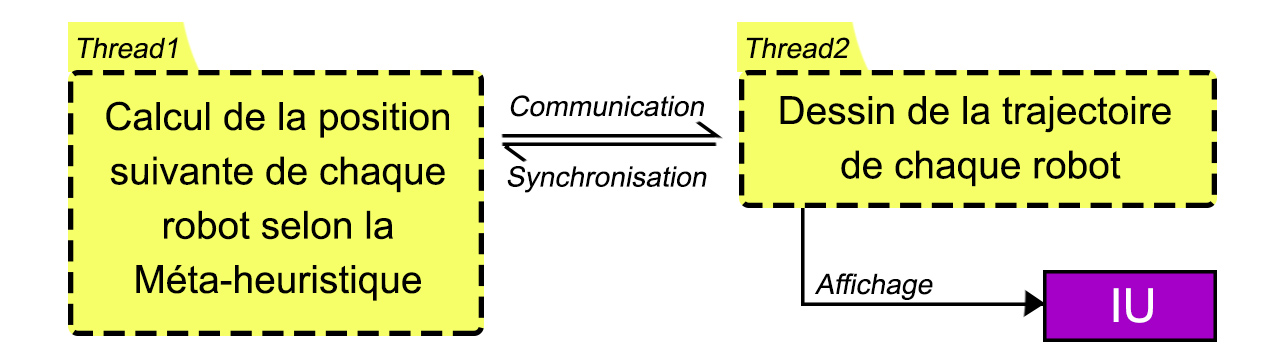
\includegraphics[width=0.8\textwidth]{threads.jpg}%
	\captionof{figure}{Schéma de communication du système multi-threads.}\label{sim}%
\end{center}



\subsection{Interface}
L'interface offrent deux sections possibles celle dédiés au choix de l'environnement nous permettant de choisir un environnement selon nos préférences et paramètres, et une autre section dédiées aux métaheuristiques, celle-ci englobe toutes les approches basées essaims que nous avons traité dans ce projet appliquées à l'environnement choisi dans la section Environnement.
Les deux sections sont visibles dans l'annexe \ref{AppendixC}.

\subsubsection{Environnement}
La section Environnement permet à l'utilisateur de choisir un environnement selon les paramètres et préférences suivantes :

\paragraph{Portée des cibles}
Les cibles recherchées par nos robots peuvent être très variées d'où la nécessité de proposer des cibles à portée variantes, ainsi on pourra observer les comportements des approches basées essaims sur chaque type. Les portées de cibles disponibles dans l'application sont donc catégorisées comme suit:
\vspace{0.3cm}
\begin{itemize}
	\item [$\bullet$] \textbf{Portée petite}, d'un rayon d'environ 5\% de la taille de l'environnement.
	\item [$\bullet$] \textbf{Portée moyenne}, d'un rayon d'environ 15\% de la taille de l'environnement.
	\item [$\bullet$] \textbf{Portée large}, d'un rayon d'environ 25\% de la taille de l'environnement.
\end{itemize}


\paragraph{Nombre de cibles}
Le nombre de cibles est aussi un paramètres qui influe les approches implémentés, ainsi pour des soucis de visualisation nous nous sommes contenté de permettre deux choix uniquement pour le nombre de cibles qui sont:
\begin{itemize}
	\item [$\bullet$] Mono-cible : une seule cible.
	\item [$\bullet$] Multi-cibles avec 5 cibles.
\end{itemize}
Ce choix peut être augmenté selon les environnements qu'on souhaite avoir selon le nombre de cibles voulu.

\paragraph{Type d'environnement}
Le choix des types d'environnements est exactement le même que vu dans le chapitre 3 ainsi que dans les expérimentations du chapitre 4. Soient:

\begin{table}[h]
	\centering
	\begin{tabular}{|c|c|c|} 
		\hline
		Simple &  Obstacles & Complexe \\
		\hline
		%\bottomrule
	\end{tabular}
	\captionsetup{width=1\linewidth}
	\vspace{-0.1cm}
	%\caption{Types d'environnement.}
	\label{TypeEnv}
\end{table}

\vspace{-0.5cm}
\paragraph{Taille d'environnement}
Les environnements varient selon leur taille, on a alors choisi à titre représentatif quelques tailles par classe, telles que:
\begin{itemize}
	\item  [$\bullet$]100 et 400 qui sont assez petits.
	\item  [$\bullet$]600 et 1000 dits moyens.
	\item  [$\bullet$]1500 qui est assez grand.
\end{itemize}

\paragraph{Afficher}
La section environnement présentée dans la figure \ref{uienvsetting} comporte le bouton \textit{afficher} qui sert à visualiser l'environnement choisi en fonction des préférences insérées dans les listes de choix multiples de chaque influent (portée,nombre cibles,...). 

Ci-dessous un exemple d'environnement sélectionné:
\begin{center}	  
	\captionsetup{width=1\linewidth}
	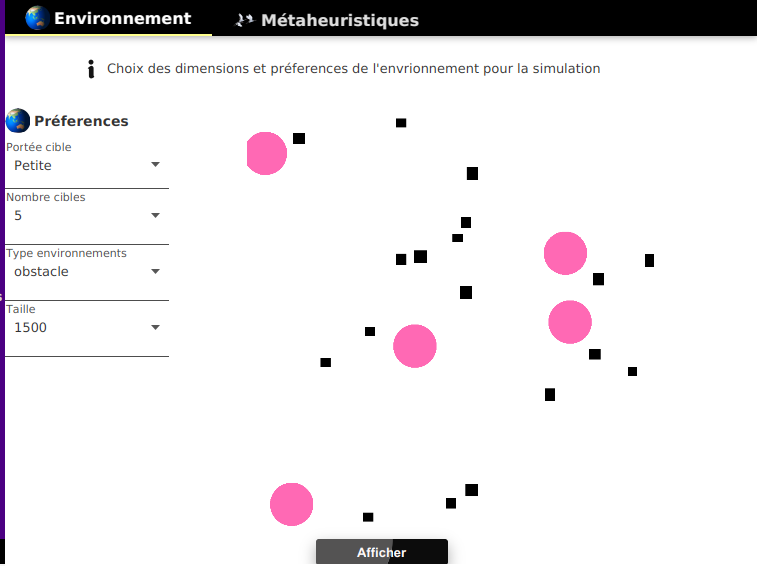
\includegraphics[scale=0.45]{screens/envsetting.png}%
	\vspace{-0.1 cm}
	\captionof{figure}{Affichage de l'environnement selon les préférences insérées}\label{uienvsetting}%
\end{center}

\subsubsection{Métaheuristiques}

\paragraph{Les approches}
Les approches basées essaims aux quelles nous avons eu affaire tout au long de ce mémoire \textit{BSO, EHO, ESWSA, Multi-BSO} y sont proposées sous forme d'une liste permettant de choisir celle à exécuter.
Une fois qu'on clique sur une approche deux possibilités s'offrent à nous pour le choix du paramétrage:


\paragraph{- Paramétrage avec algorithme génétique}
L'option de paramétrage avec l'algorithme génétique (Mini-GA incrémental) est accessible pour chaque approche, comme le montre la figure \ref{uiga} ci-dessous.

\begin{center}	  
	\captionsetup{width=1\linewidth}
	\includegraphics[scale=0.5]{screens/bsoautoparam.png}%
	\vspace{-0.1 cm}
	\captionof{figure}{Auto-paramétrage avec l'algorithme génétique}\label{uiga}%
\end{center}

\paragraph{- Paramétrage manuel}
Le paramétrage manuel se fait en choisissant pour chaque paramètre de l'approche basée essaim une valeur.
Les figures \ref{uibso} et \ref{uibsoga} suivantes illustrent ces paramètres pour BSO.

\begin{minipage}{0.5\textwidth}
	\centering
	\includegraphics[scale=0.50]{screens/bsopopmenu.png}%
	\vspace{-0.1 cm}
	\captionof{figure}{Menu de paramétrage}\label{uibso}%
\end{minipage}%
\begin{minipage}{0.5\textwidth}
	\centering	  
	\captionsetup{width=0.6\linewidth}
	\includegraphics[scale=0.40]{screens/bsoparam20-2-3.png}%
	\vspace{-0.1 cm}
	\captionof{figure}{Menu de paramétrage manuel pour BSO}\label{uibsoga}%
\end{minipage}

\textbf{ }\\

\noindent
\begin{minipage}{0.6\textwidth}
\paragraph{Les informations}
Ce sont les détails identiques pour chaque approche et qui sont:
\textit{Nombre d'itérations, Nombre de cibles trouvées, Temps d'exécution (sec)} comme présentés dans la figure \ref{bsoinfo}.

Ces informations sont mises à jour en temps réel, c'est à dire elles sont modifiés à chaque itération (le nombre d'itération inclus).
\end{minipage}
\begin{minipage}{0.4\textwidth}
	\captionsetup{width=0.7\linewidth}
	\centering
	\includegraphics[scale=0.55]{screens/bsoinfo.png}%
	\vspace{-0.1 cm}
	\captionof{figure}{Informations durant l'exécution de BSO}\label{bsoinfo}%
\end{minipage}





\paragraph{Paramétrage}
Consiste en une liste horizontale représentée dans l'illustration \ref{listparam}, elle contient les paramètres de l'exécution de l'approche choisie, qu'elle soit générée par algorithme génétique ou bien manuellement à travers le menu de paramétrage manuel vu plus haut.


\begin{center}	  
	\captionsetup{width=1\linewidth}
	\includegraphics[scale=0.65]{screens/bsoparamlist.png}%
	\vspace{-0.1 cm}
	\captionof{figure}{Liste des paramètres pour BSO}\label{listparam}%
\end{center}


\paragraph{Les boutons}
\textbf{ }\\
Notre interface comporte deux boutons qui se trouvent à côté du "slider".
\paragraph{-Start}
Le bouton \textit{"Start"} \includegraphics[scale=0.55]{screens/start.png} , permet de débuter l'exécution après avoir choisi l'approche.
Ainsi l'image de l'environnement et des robots (abeilles ou éléphants) sur l'environnement s'affichent.


\paragraph{-Stop}
Le bouton \textit{"Stop"}	\includegraphics[scale=0.55]{screens/stop.png}, permet d'arrêter et mettre fin à l'exécution de l'approche, afin de choisir une autre Méta à exécuter ou bien relancer la même avec d'autres paramètres.


\paragraph{Le slider} de la figure \ref{slider} joue le rôle d'une barre de progression, tel qu'il s'incrémente après chaque itération de l'approche en cours d'exécution. Une fois l'exécution terminée, il permet de revenir en arrière retraçant ainsi la trajectoire des robots dans l'environnement. Comme pour un film ou une vidéo nous avons la possibilité d'avancer du début jusqu'à la fin, pour revoir l'exécution.

\begin{center}	  
	\captionsetup{width=1\linewidth}
	\includegraphics[scale=0.55]{screens/slider.png}%
	\vspace{-0.1 cm}
	\captionof{figure}{Le slider}\label{slider}%
\end{center}

L'illustration \ref{bsorun} suivante est un exemple d'une exécution de BSO dans un environnement multi-cibles de petites portées et avec obstacles.
\begin{center}	  
	\captionsetup{width=1\linewidth}
	\includegraphics[scale=0.45]{screens/bsorun20-2-3.png}%
	\vspace{-0.1 cm}
	\captionof{figure}{Exemple d'exécution de BSO.}\label{bsorun}%
\end{center}


\paragraph{Quitter}
Un bouton quitter (voir figure \ref{exit}) se trouve en bas à gauche de l'interface afin de sortir de l'application dès que nous le souhaitons.

\begin{center}	  
	\captionsetup{width=1\linewidth}
	\includegraphics[scale=0.8]{screens/exit.png}%
	\vspace{-0.1 cm}
	\captionof{figure}{Bouton pour quitter l'application}\label{exit}%
\end{center}




\section{Conclusion}
Dans ce dernier chapitre, nous avons présenté les résultats de tous les testes effectués sur nos méta-heuristiques, entre les tests expérimentales pour leurs paramétrages avec l'algorithme génétique ( nombre indéterminé d'exécutions) et les expérimentations relatives aux caractéristiques de l'environnement soient : Portée, taille, nombre de cible, type d'environnement (23 040 exécutions).

Cela nous a permis de trouver les points forts et les points faibles de chaque approche, pour une éventuelle hybridation qui donnera lieu à un algorithme qui surpassera ceux présentés dans dans ce mémoire.\\


